% Created 2020-09-14 Mon 22:20
% Intended LaTeX compiler: pdflatex
\documentclass[11pt, reqno, oneside]{amsart}
              \newcommand\subtitle[1]{\newcommand\mrgsubtitle{#1}}
\newcommand\mrgproject{Torsten report}
\newcommand\mrgtitle{Speed up population Bayesian inference by combining cross-chain warmup and within-chain parallelism}
\newcommand\mrgsubtitle{\Large{Based on:} \linebreak (Torsten Version xxx, Stan version 2.23)}
\renewcommand\maketitle{
  \begin{titlepage}%
    \definecolor{MRGGreen}{rgb}{0, 0.350, 0.200}

    \thispagestyle{empty}

    \begin{center}
      
\includegraphics[height=0.75in]{graphics/logo.jpg}\\
      \vspace{10mm} %5mm vertical space
      \textcolor{MRGGreen}{\sf Metrum Research Group LLC \hfill 2 Tunxis Road, Suite 112} \\
      \textcolor{MRGGreen}{\sf Phone: 860.735.7043 \hfill Tariffville, CT 06081}\\
      \textcolor{MRGGreen}{\sf billg@metrumrg.com, yiz@metrumrg.com \hfill \href{http://www.metrumrg.com/}{www.metrumrg.com}}\\
      {\Huge \textcolor{MRGGreen}{\textbf{\mrgproject}} \\ \ \\  \huge{\mrgtitle} \\ \ \\ \mrgsubtitle\\ \ \\ \ \\
        
        \large \today}
    \end{center}

    \clearpage
  \end{titlepage}%
}

\usepackage{imakeidx}
\makeindex
\usepackage[letterpaper, width=6.5in, height=9in]{geometry}
\usepackage{graphicx}
\usepackage{pdfpages}
\usepackage{amssymb}
\usepackage{epstopdf}
\usepackage{xcolor}
\definecolor{MRGGreen}{rgb}{0, 0.350, 0.200}
\usepackage[colorlinks=true, citecolor=MRGGreen, urlcolor=MRGGreen, linkcolor=MRGGreen]{hyperref}
\usepackage{courier}
\usepackage{listings}
\usepackage{siunitx}
\usepackage{booktabs}
\usepackage[framemethod=TikZ, skipabove=10pt, skipbelow=10pt, backgroundcolor=black!5, roundcorner=4pt, linewidth=1pt]{mdframed}
\BeforeBeginEnvironment{minted}{\begin{mdframed}}
\AfterEndEnvironment{minted}{\end{mdframed}}


\usepackage[utf8]{inputenc}
\usepackage[T1]{fontenc}
\usepackage{graphicx}
\usepackage{grffile}
\usepackage{longtable}
\usepackage{wrapfig}
\usepackage{rotating}
\usepackage[normalem]{ulem}
\usepackage{amsmath}
\usepackage{textcomp}
\usepackage{amssymb}
\usepackage{capt-of}
\usepackage{hyperref}
\usepackage[newfloat]{minted}
\usepackage{caption}
\author{Yi Zhang}
\date{\today}
\title{Speed up population Bayesian inference by combining cross-chain warmup and within-chain parallelism}
\hypersetup{
 pdfauthor={Yi Zhang},
 pdftitle={Speed up population Bayesian inference by combining cross-chain warmup and within-chain parallelism},
 pdfkeywords={},
 pdfsubject={},
 pdfcreator={Emacs 26.3 (Org mode 9.1.9)}, 
 pdflang={English}}
\begin{document}

\maketitle

\section{Introduction}
\label{sec:orga196c19}
With increasing adoption of Bayesian inference to
pharmacometric(PMX) modeling, it has become evident that
high-performance computing(HPC) must be utilized for large-scale
models to be accessible, and inference framework based on Markov Chain
Monte Carlo(MCMC) must improve efficiency through multiple
channels. For example, probabilistic programming language Stan \cite{carpenter_stan_2017}
uses efficient samplers such as the No-U-Turn
Sampler(NUTS) \cite{hoffman_no-u-turn_2014}, and provide \mintinline[breaklines=true,fontsize=\footnotesize,breakanywhere=true]{stan}{map_rect} functions
to parallelize expensive likelihood evaluation.

The scope of the work presented here is to improve Bayesian inference
efficiency of population models. The work is based on Torsten
\cite{Torsten}, a library of Stan functions that
simplifies PMX modeling and
extends the range of models that may be implemented. We address two
aspects of the efficiency problem. First, we propose a dynamic warmup
approach, as an alternative to current Stan's warmup where a fixed
number(default 1000) of iterations are performed. Second, we combine
the new warmup algorithm with existing within-chain parallelization
functionality of Torsten \cite{torsten_pmx_group} to formulate a \emph{multilevel} parallel method
that utilizes dynamic warmup \emph{and} within-chain parallelism to speed
up simulation.

\section{Cross-chain warmup}
\label{sec:org5b4c5f7}
\subsection{Algorithm \& implementation}
\label{sec:orgf690079}
The standard practice of Stan is to perform a fixed number of warmup
iterations. With this practice, the efficacy of the warmup is unknown
\emph{a priori} and often warmup is unncessarily long as user oversubscribe warmup iterations.
The proposed warmup algorithm tries to avoid this by checking potential scale reduction
coefficients (\(\hat{R}\)) and effective sample sizes (ESS)
\cite{vehtari_rank-normalization_2019} . Specifically, for warmup we
propose(see also Figure \ref{cc-diagram}).
\begin{figure}[htbp]
\centering
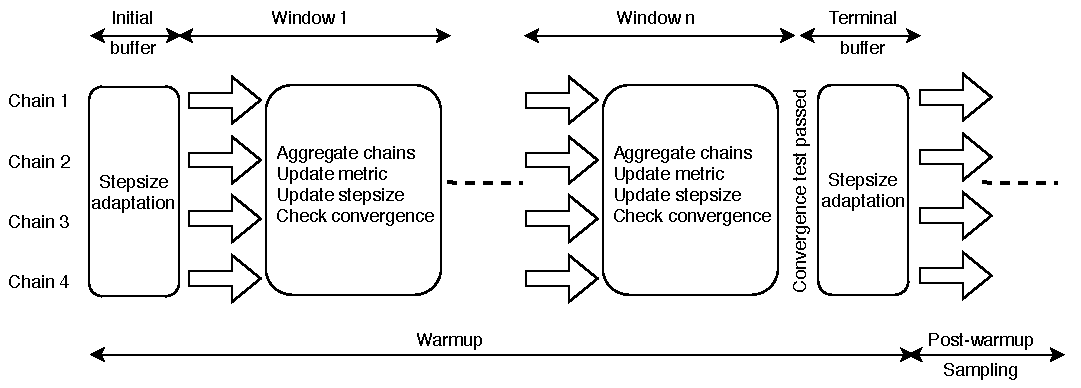
\includegraphics[width=\textwidth]{./figure/cross_chain_diagram.pdf}
\caption{Cross-chain warmup algorithm \label{cc-diagram}}
\end{figure}

\begin{enumerate}
\item Given a fixed window size \(w\)(default 100) and initial buffer size(default 75), the sampler iterates during warmup with stepsize adapted as in regular warmup runs.
\item At the end of a window, we aggregate the joint posterior probability \texttt{lp\_\_} from all the chains and calculate corresponding \(\hat{R}\) as well as ESS. 
Specifically, when the warmup reaches the last iteration of window
\(n\), we calculate \(\hat{R}^i\) and \(\text{ESS}^i\), \(i=1\dots,n\). The
superscript \(i\) indicates that the quantity is calculated based on
\texttt{lp\_\_} aggregated from all the chains, using the iterations from
window \(i\), \(i+1\), \dots{}, \(n\). For example, with default window
size \(w=100\), when warmup reaches iteration 300, we calculate
\(\hat{R}^i\) and \(\text{ESS}^i\) for \(i=1, 2, 3\), so that

\(\hat{R}^1\) and \(\text{ESS}^1\) are based on warmup iteration 1 to 300;

\(\hat{R}^2\) and \(\text{ESS}^2\) are based on warmup iteration 101 to 300;

\(\hat{R}^3\) and \(\text{ESS}^3\) are based on warmup iteration 201 to 300.

\item At the end of window \(n\), with predefined target value \(\hat{R}^{0}\) and ESS\(^{0}\), from \({1, \dots, n}\),  we select \(j\) such that
\begin{equation}
\text{ESS}^j > \text{ESS}^i,\quad \forall i\neq j, \quad 1\le i\le n.
\end{equation}
Namely, we select \(j\) so that it has the maximum ESS. A new metric
is calculated by aggregating samples from

\begin{equation*}   
   \text{window } j, \text{window } j+1, ..., \text{window } n
\end{equation*}
from all the chains, and a new stepsize is calculated by taking geometric mean
of chain stepsizes. The new metric and stepsize are used in future iterations for all the chains.
If, in addition, \(j\) satisfies
\begin{equation}
\begin{aligned}
\hat{R}^j < \hat{R}^0,\\
\text{ESS}^j > \text{ESS}^0,
\end{aligned}
\end{equation}
the warmup is considered complete((\emph{converges}). Otherwise warmup continues until
the end of the next window and step 2-3 are repeated.
\item After convergences, the warmup
continues into terminal buffer(50 iterations by default). As in
standard Stan warmup, in this buffer the metric is no longer
updated while stepsize is further adapted.
\end{enumerate}

Unlike current warmup scheme, the above proposal requires
communication among the chains, hence we call it \emph{cross-chain warmup}.
The implementation is based on Torsten's parallel setup using Message
Passing Interface (MPI). In
a cross-chain warmup run, all chains move forward independently except
at the end of a window, where samples are aggregated from the chains
to calculate \(\hat{R}^i\) and ESS\(^i\) and new metric and stepsize are
distributed to the chains.
After warmup the sampler moves into independent post-warmup sampling stage
with no more cross-chain communications.

The latest version of cross-chain warmup implementation can be found
at

\subsection{Performance evaluation}
\label{sec:orgeefee9a}
We compare the two warmup schemes by running several models
from \href{https://github.com/MansMeg/posteriordb}{posteriordb} and \href{https://github.com/metrumresearchgroup/Torsten/tree/master/example-models}{Torsten} repo. For each model, we compare the
effect of warmup on 
\begin{itemize}
\item total number of leapfrog integration steps in warmup
\item total number of leapfrog integration steps in sampling
\item number of leapfrog integration steps in per each warmup iteration
\item number of leapfrog integration steps in per each sampling iteration
\item minimum ESS\(_{\text{bulk}}\) per iteration
\item minimum ESS\(_{\text{tail}}\) per iteration
\item minimum ESS\(_{\text{bulk}}\) per leapfrog step
\item minimum ESS\(_{\text{tail}}\) per leapfrog step
\item maximum wall time
\end{itemize}

We run each model runs with 10 random seeds 
\begin{minted}[breaklines=true,fontsize=\footnotesize,breakanywhere=true]{r}
seed <- seq(8235121, 8235130)
\end{minted}
and plot the above
quantities' the average(barplot)
and standard deviation(error bar).

For a \mintinline[breaklines=true,fontsize=\footnotesize,breakanywhere=true]{r}{stanfit} object, we use the following R
function evaluate cross-chain performance.
\begin{minted}[breaklines=true,fontsize=\footnotesize,breakanywhere=true]{r}
## Based on Aki's script to evaluate ESS
perf.cc <- function(stanfit) {
    (n_chain = stanfit@sim$chains)
    (n_warmup = stanfit@sim$warmup)
    n_iter = stanfit@sim$iter-n_warmup
    sampler_params <- rstan:::get_sampler_params(stanfit, inc_warmup = TRUE)
    leapfrogs = sapply(sampler_params, function(x) x[, "n_leapfrog__"])
    (sum_warmup_leapfrogs = sum(leapfrogs[1:n_warmup,]))
    (sum_leapfrogs = sum(leapfrogs[n_warmup+(1:n_iter),]))
    (mean_warmup_leapfrogs = sum_warmup_leapfrogs/n_warmup / n_chain)
    (mean_leapfrogs = sum_leapfrogs/n_iter / n_chain)
    mon = rstan::monitor(as.array(stanfit), warmup=0, print=FALSE)
    (maxrhat = max(mon[,'Rhat']))
    bulk_ess_per_iter = mon[,'Bulk_ESS']/n_iter / n_chain
    tail_ess_per_iter = mon[,'Tail_ESS']/n_iter / n_chain
    bulk_ess_per_leapfrog = mon[,'Bulk_ESS']/sum_leapfrogs
    tail_ess_per_leapfrog = mon[,'Tail_ESS']/sum_leapfrogs
    min(bulk_ess_per_iter)
    min(tail_ess_per_iter)
    min(bulk_ess_per_leapfrog)
    min(tail_ess_per_leapfrog)
    elapsed <- as.data.frame(rstan::get_elapsed_time(stanfit))
    (stepsizes = sapply(sampler_params, function(x) x[, "stepsize__"])[n_iter,])

    res <- data.frame(run = c(sum_warmup_leapfrogs / n_chain, sum_leapfrogs / n_chain,
                                   mean_warmup_leapfrogs, mean_leapfrogs,
                                   min(bulk_ess_per_iter),
                              min(tail_ess_per_iter),
                              min(bulk_ess_per_leapfrog),
                              min(tail_ess_per_leapfrog),
                              max(elapsed$warmup + elapsed$sample)))
    row.names(res) <- c("leapfrogs(warmup)", "leapfrogs(sampling)",
                        "leapfrogs(warmup)/iter", "leapfrogs(sampling)/iter",
                        "min(bulk_ESS/iter)", "min(tail_ESS/iter)",
                        "min(bulk_ESS/leapfrog)", "min(tail_ESS/leapfrog)",
                        "max(elapsed_time)")
    return(res)
}
\end{minted}

For profiling cross-chain performance of a particular model, we compare
fit results from different target ESS as well as regular runs(4 chains
with 1000 warmup iterations in each chain). Figures in this section
are generated by
\begin{minted}[breaklines=true,fontsize=\footnotesize,breakanywhere=true]{r}
multiple.run.ess("cmdstan/examples", "model-name", 4, 4, "hostfile", seq(8235121, 8235130), c(100,200,400))
\end{minted}
See \mintinline[breaklines=true,fontsize=\footnotesize,breakanywhere=true]{bash}{script/run_cc.R} for details of
functions. Equivalently, one can run the model using accompanying \mintinline[breaklines=true,fontsize=\footnotesize,breakanywhere=true]{bash}{cmdstan}.
To activate cross-chain feature, compile model with \mintinline[breaklines=true,fontsize=\footnotesize,breakanywhere=true]{bash}{cmdstan/make/local} set as
\begin{minted}[breaklines=true,fontsize=\footnotesize,breakanywhere=true]{bash}
STANC2=true
MPI_ADAPTED_WARMUP=1
TBB_CXX_TYPE=clang
\end{minted}
and run it with
\begin{minted}[breaklines=true,fontsize=\footnotesize,breakanywhere=true]{bash}
# we use MPICH options in this report.
mpiexec -n 4 -l -f hostfile ./model-name sample save_warmup=1 adapt cross_chain_ess=target_ess data file=model-name.data.R init=init.R random seed=seed id=i
\end{minted}
For regular run the model should be compiled with \mintinline[breaklines=true,fontsize=\footnotesize,breakanywhere=true]{bash}{cmdstan/make/local} set as
\begin{minted}[breaklines=true,fontsize=\footnotesize,breakanywhere=true]{bash}
STANC2=true
\end{minted}
All wall time in this report are measured in seconds.

\begin{figure}[htbp]
\centering
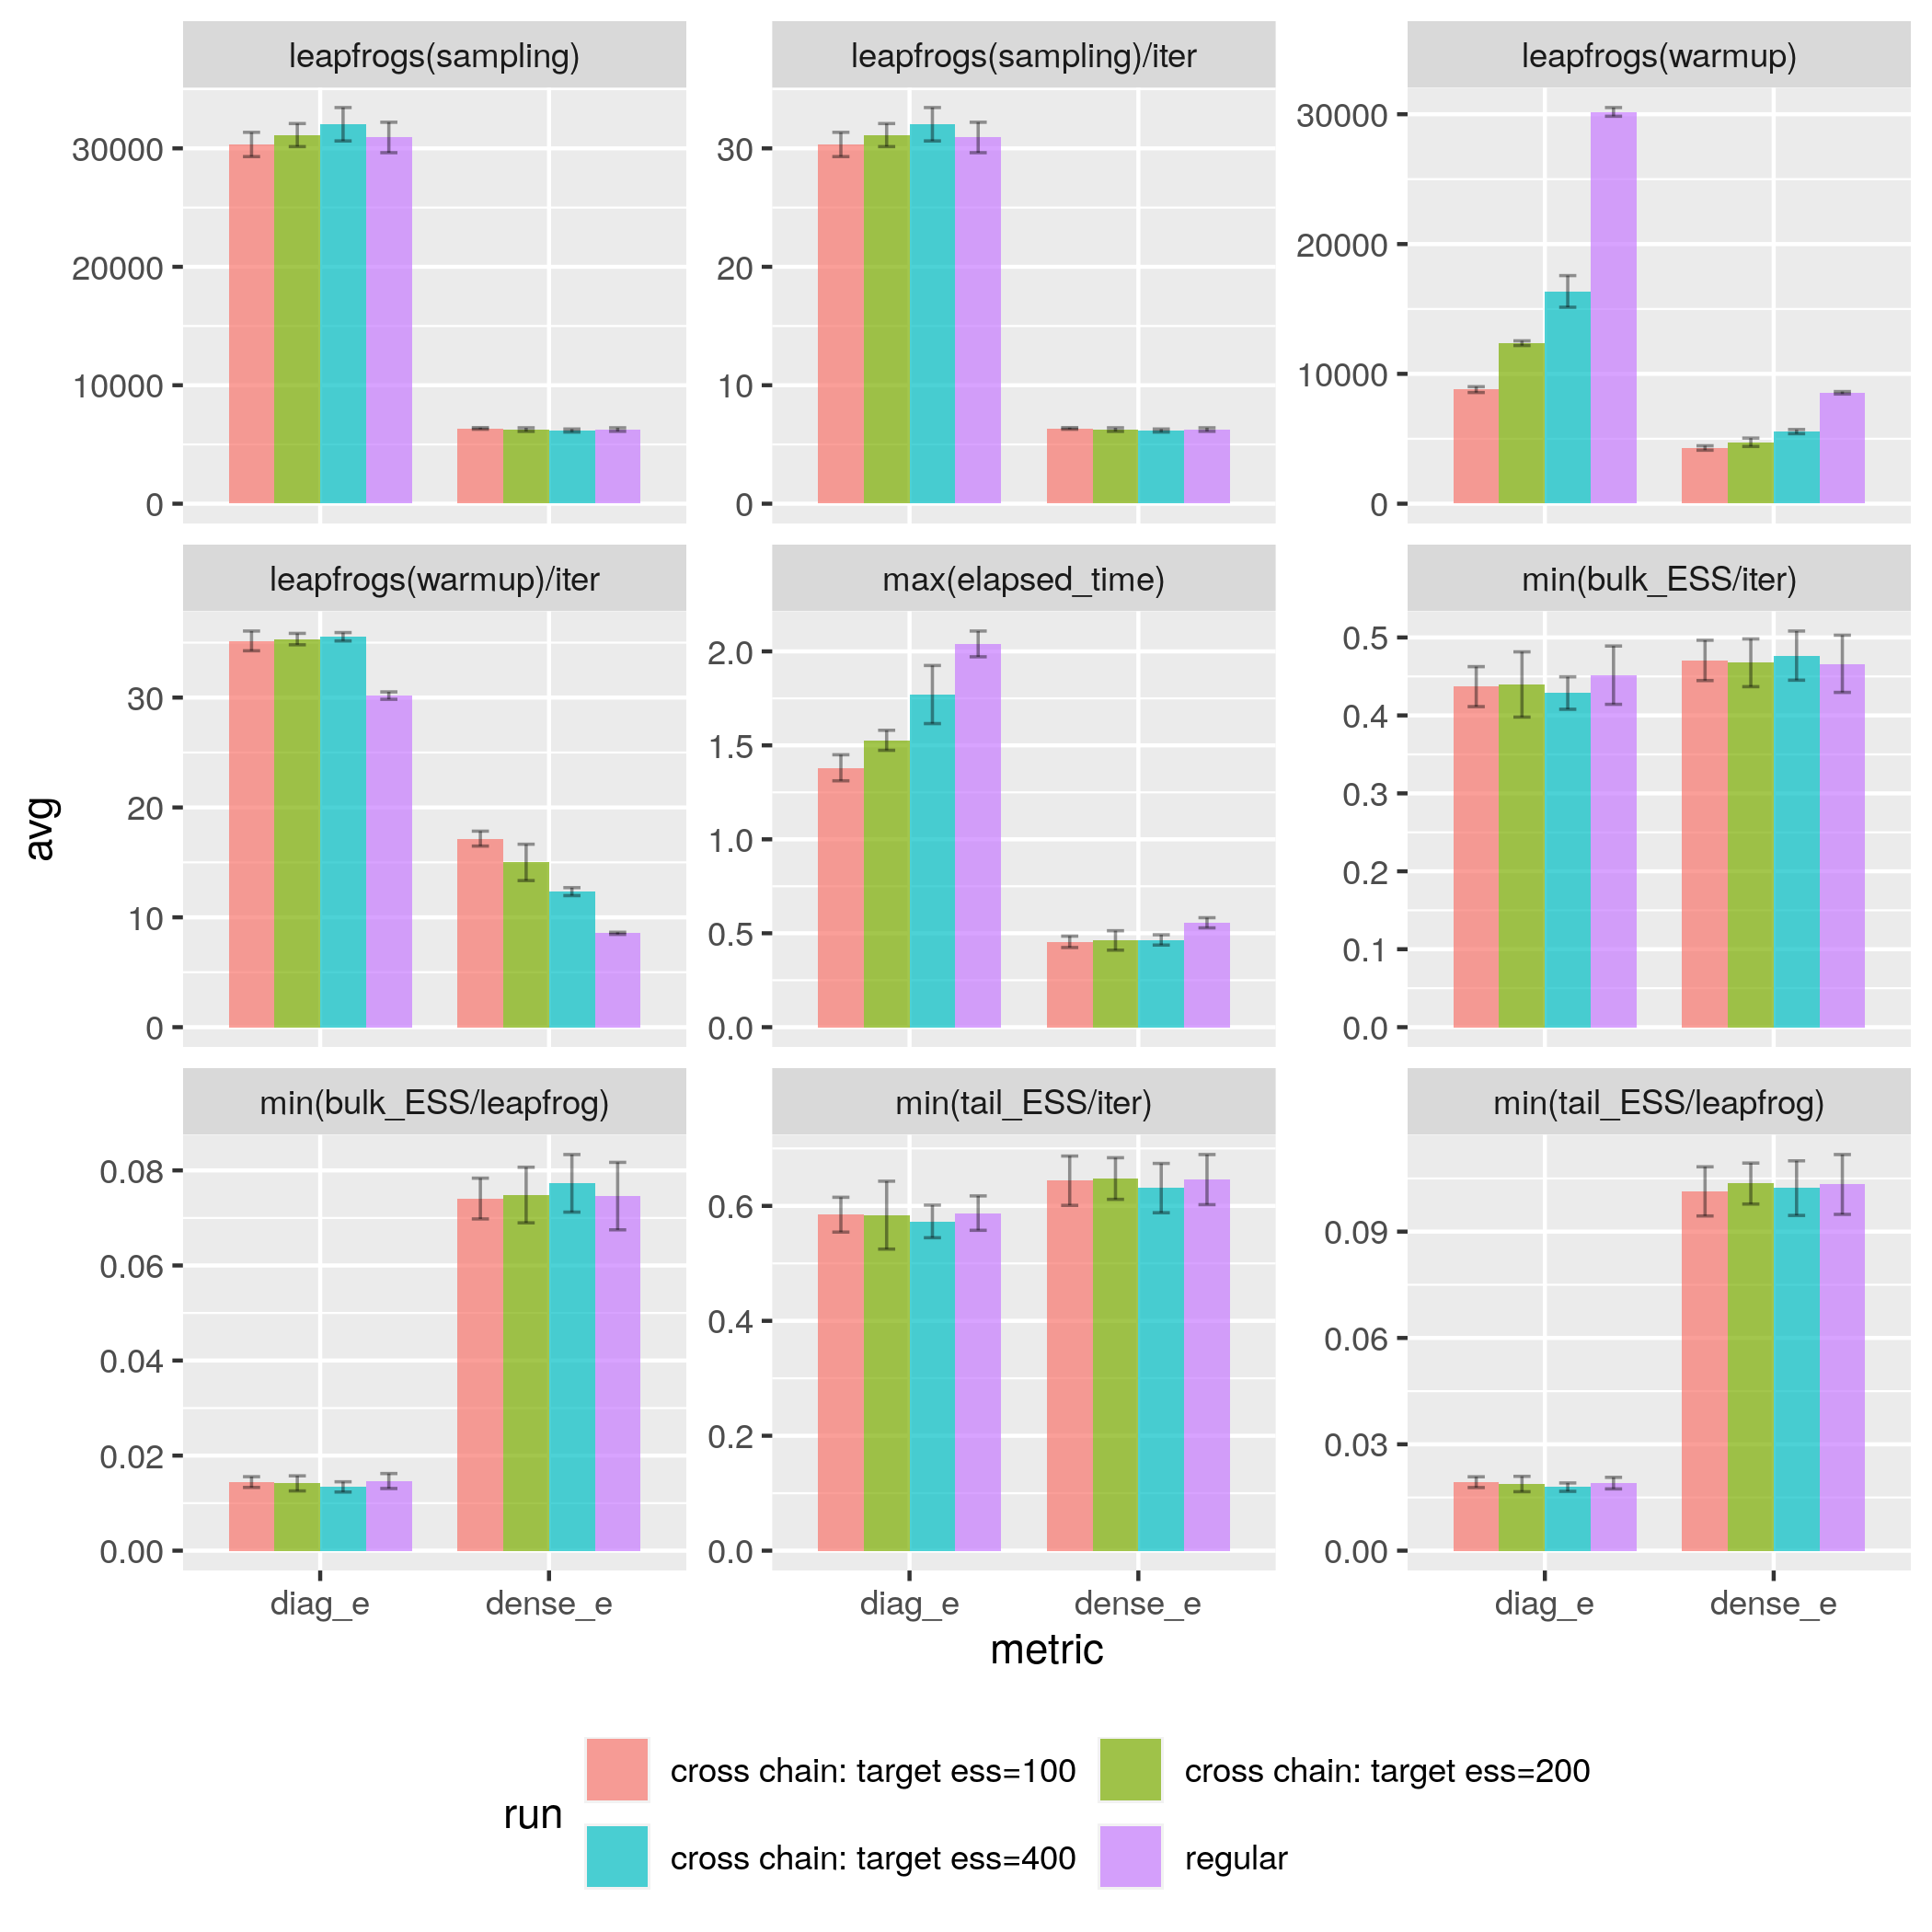
\includegraphics[width=\textwidth]{./figure/cross_chain_ess_effect_arK.png}
\caption{Cross-chain warmup performance comparison: arK model}
\end{figure}

\begin{figure}[htbp]
\centering
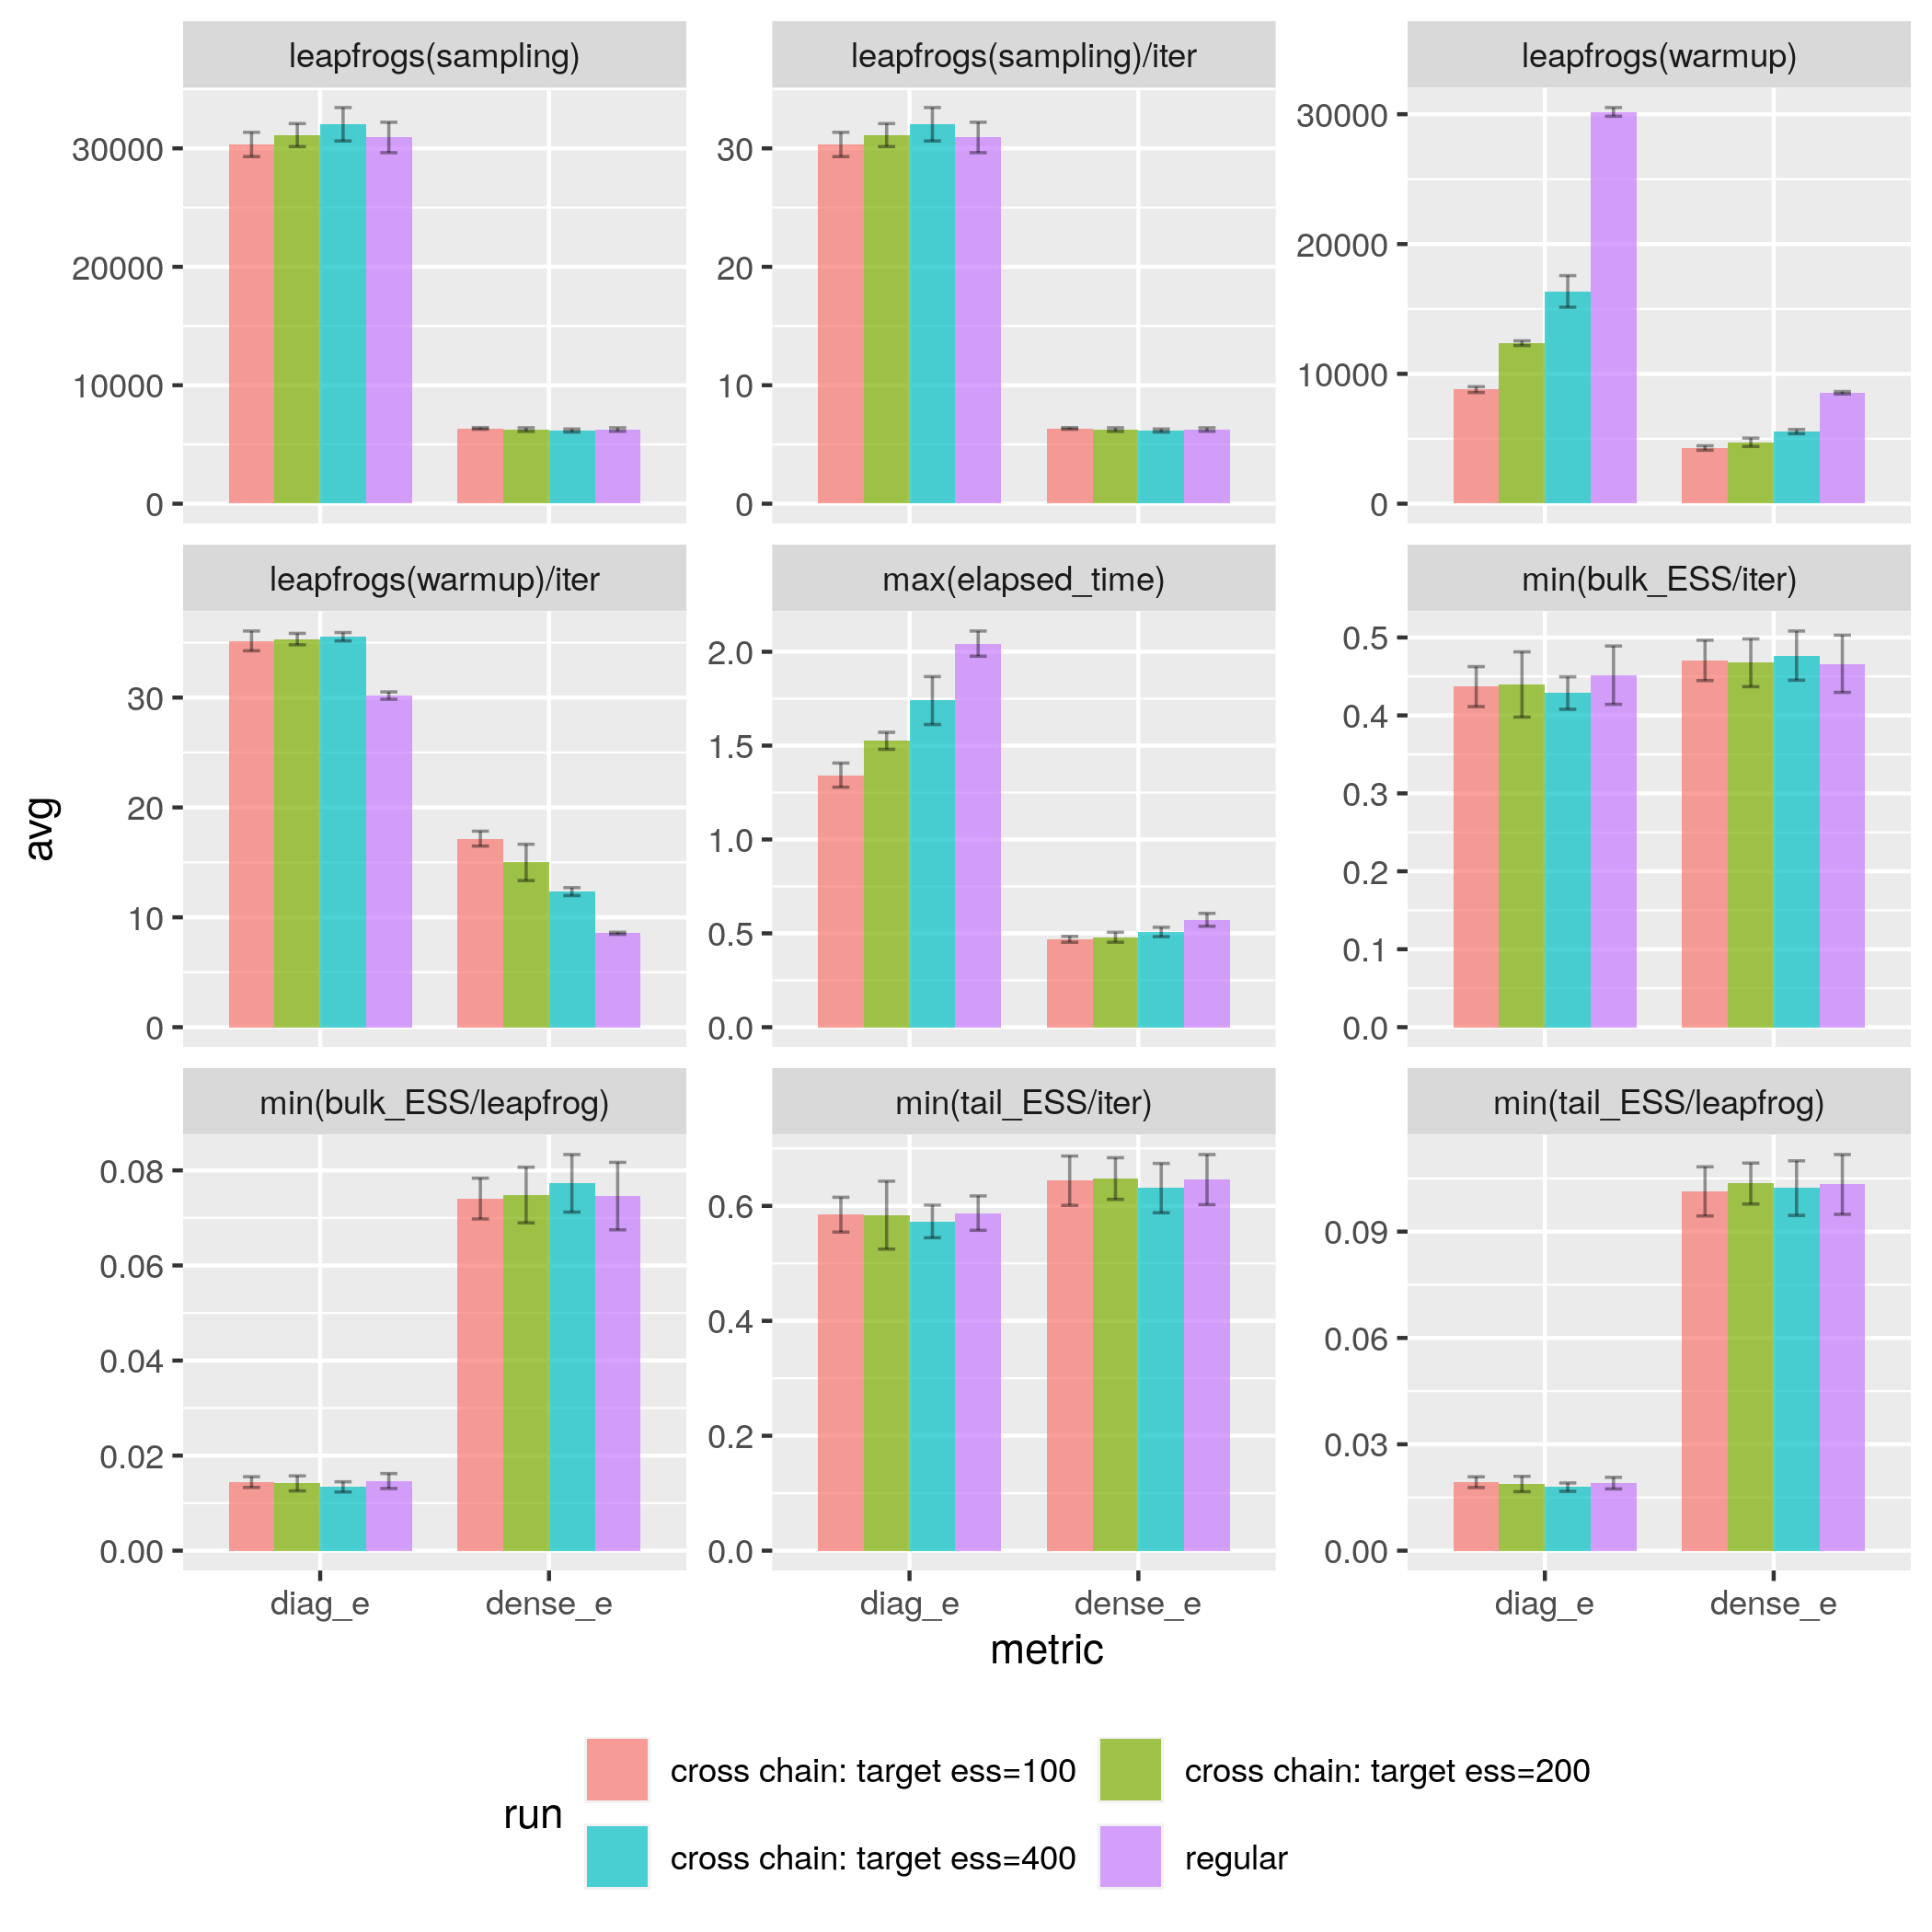
\includegraphics[width=\textwidth]{./figure/cross_chain_ess_effect_arK-arK.png}
\caption{Cross-chain warmup performance comparison: arK-arK model}
\end{figure}

\begin{figure}[htbp]
\centering
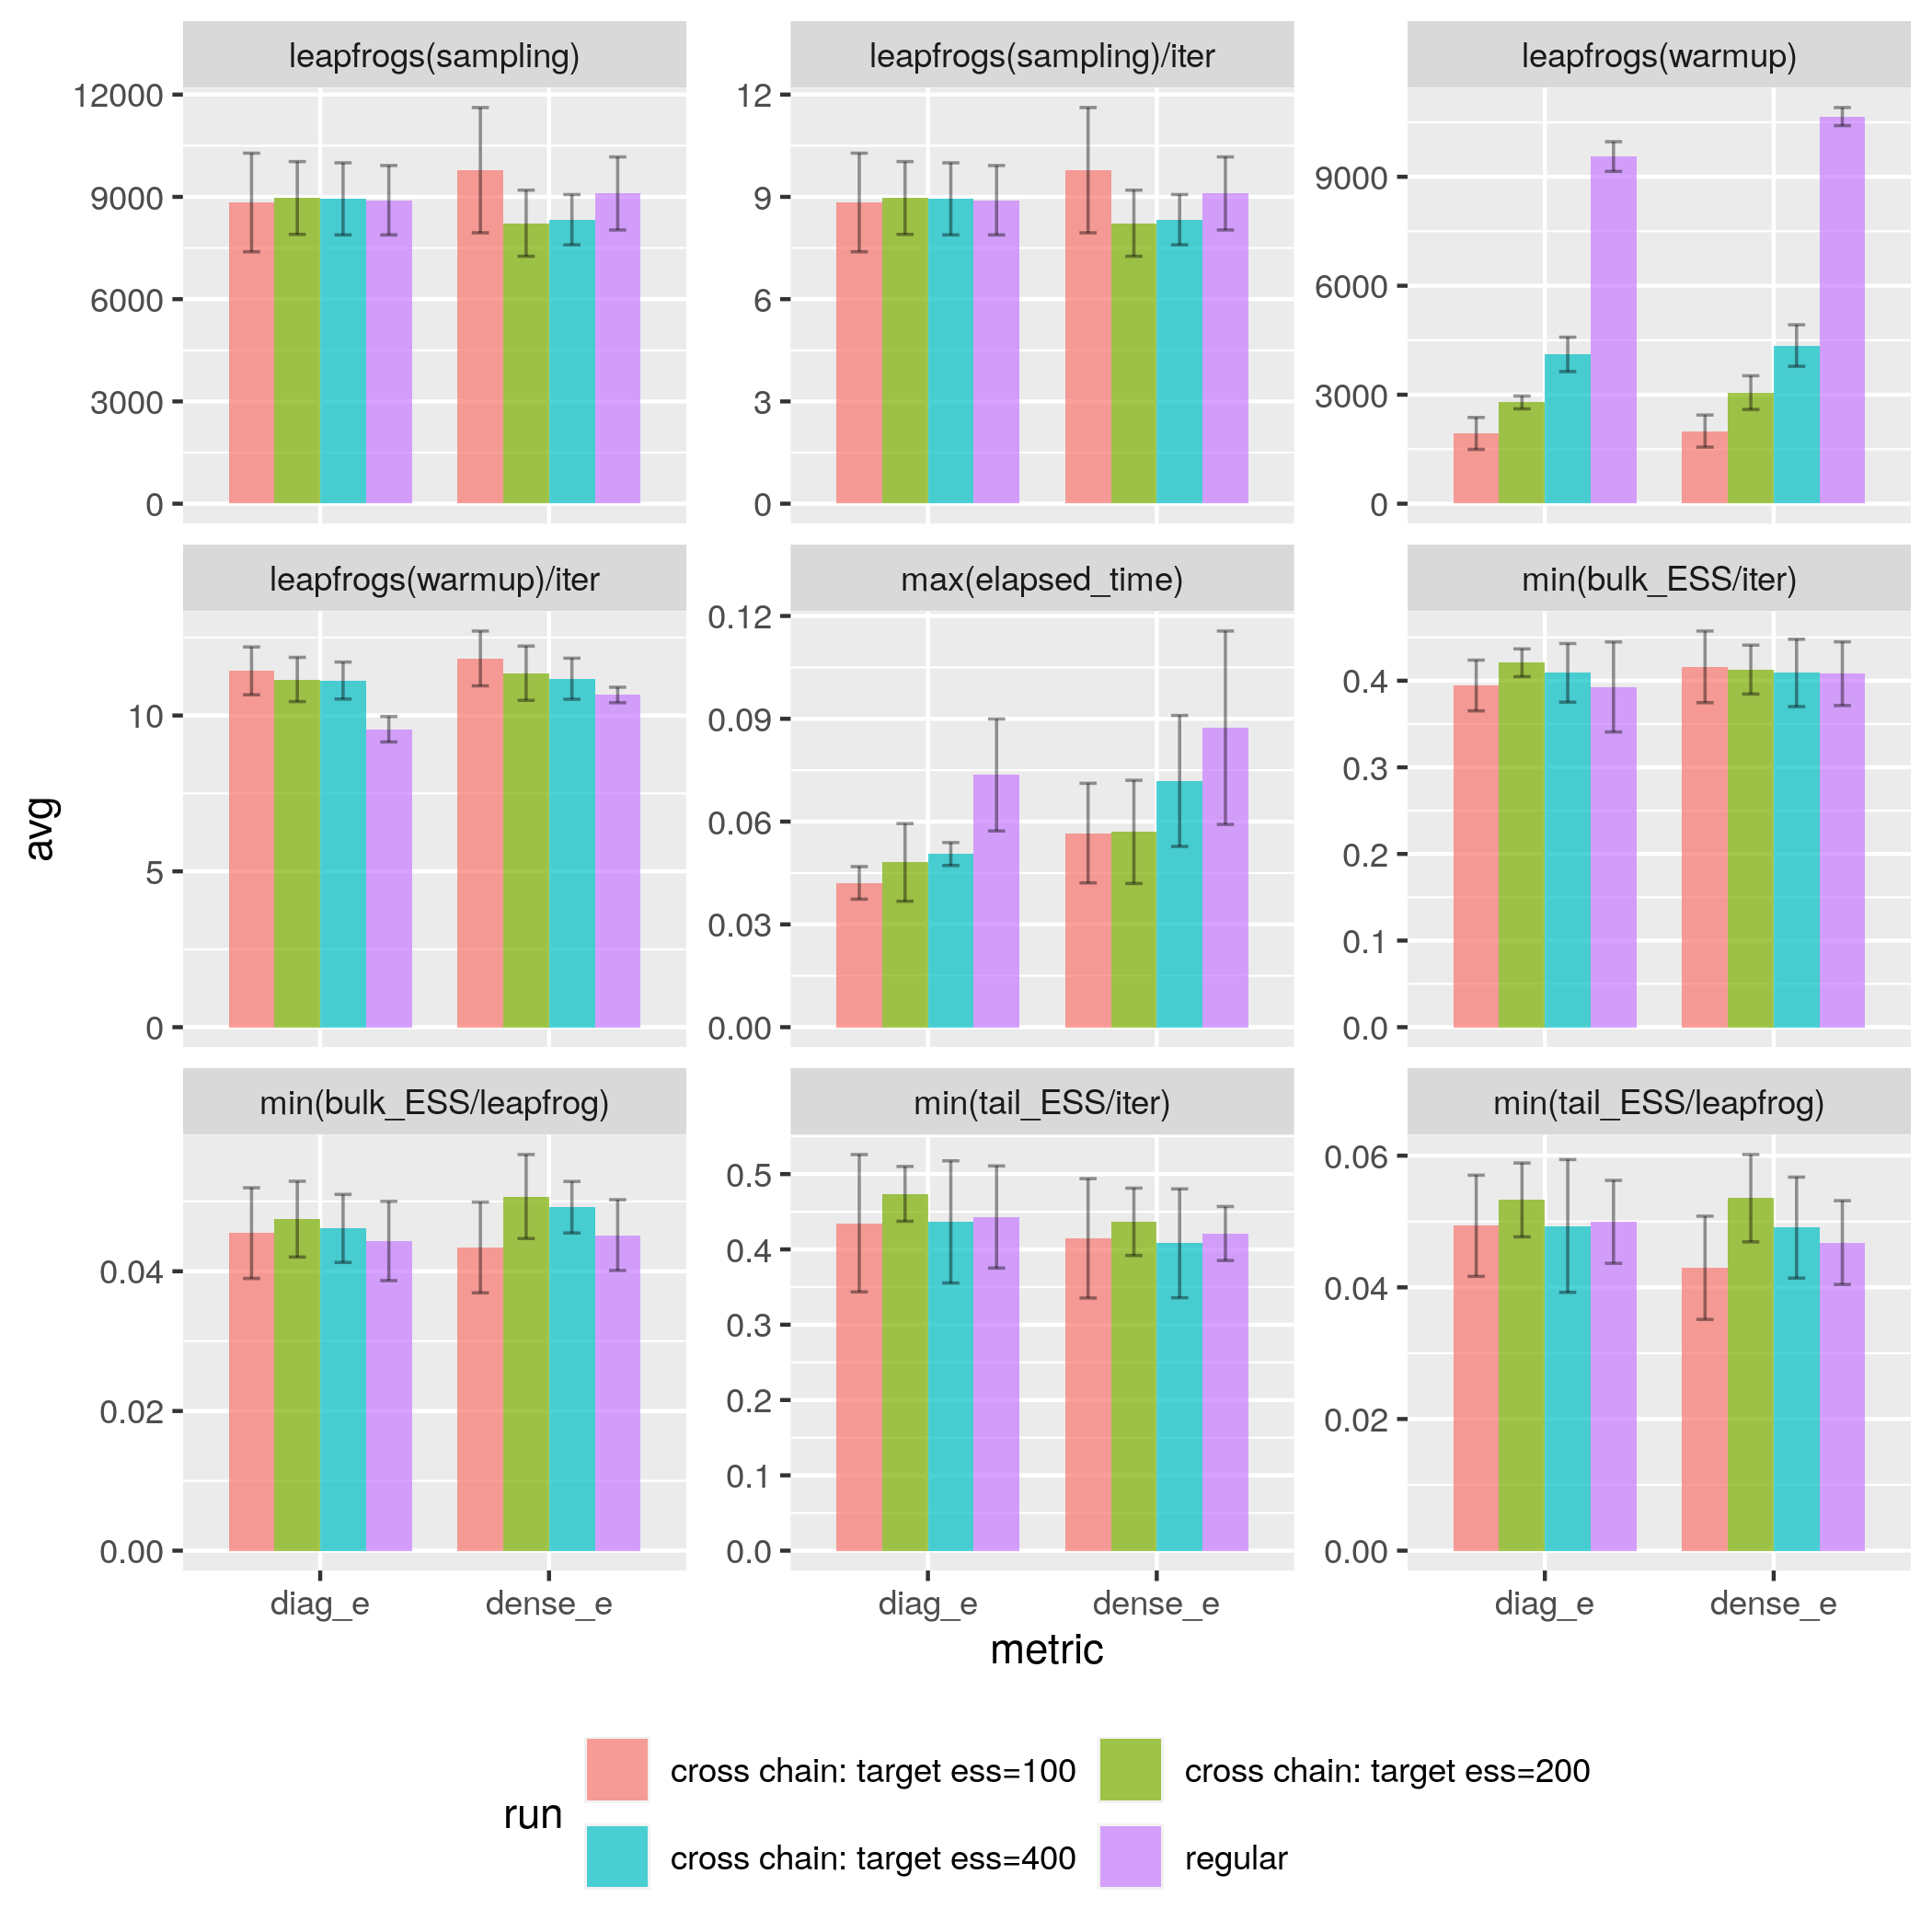
\includegraphics[width=\textwidth]{./figure/cross_chain_ess_effect_eight_schools.png}
\caption{Cross-chain warmup performance comparison: eight schools model}
\end{figure}

\begin{figure}[htbp]
\centering
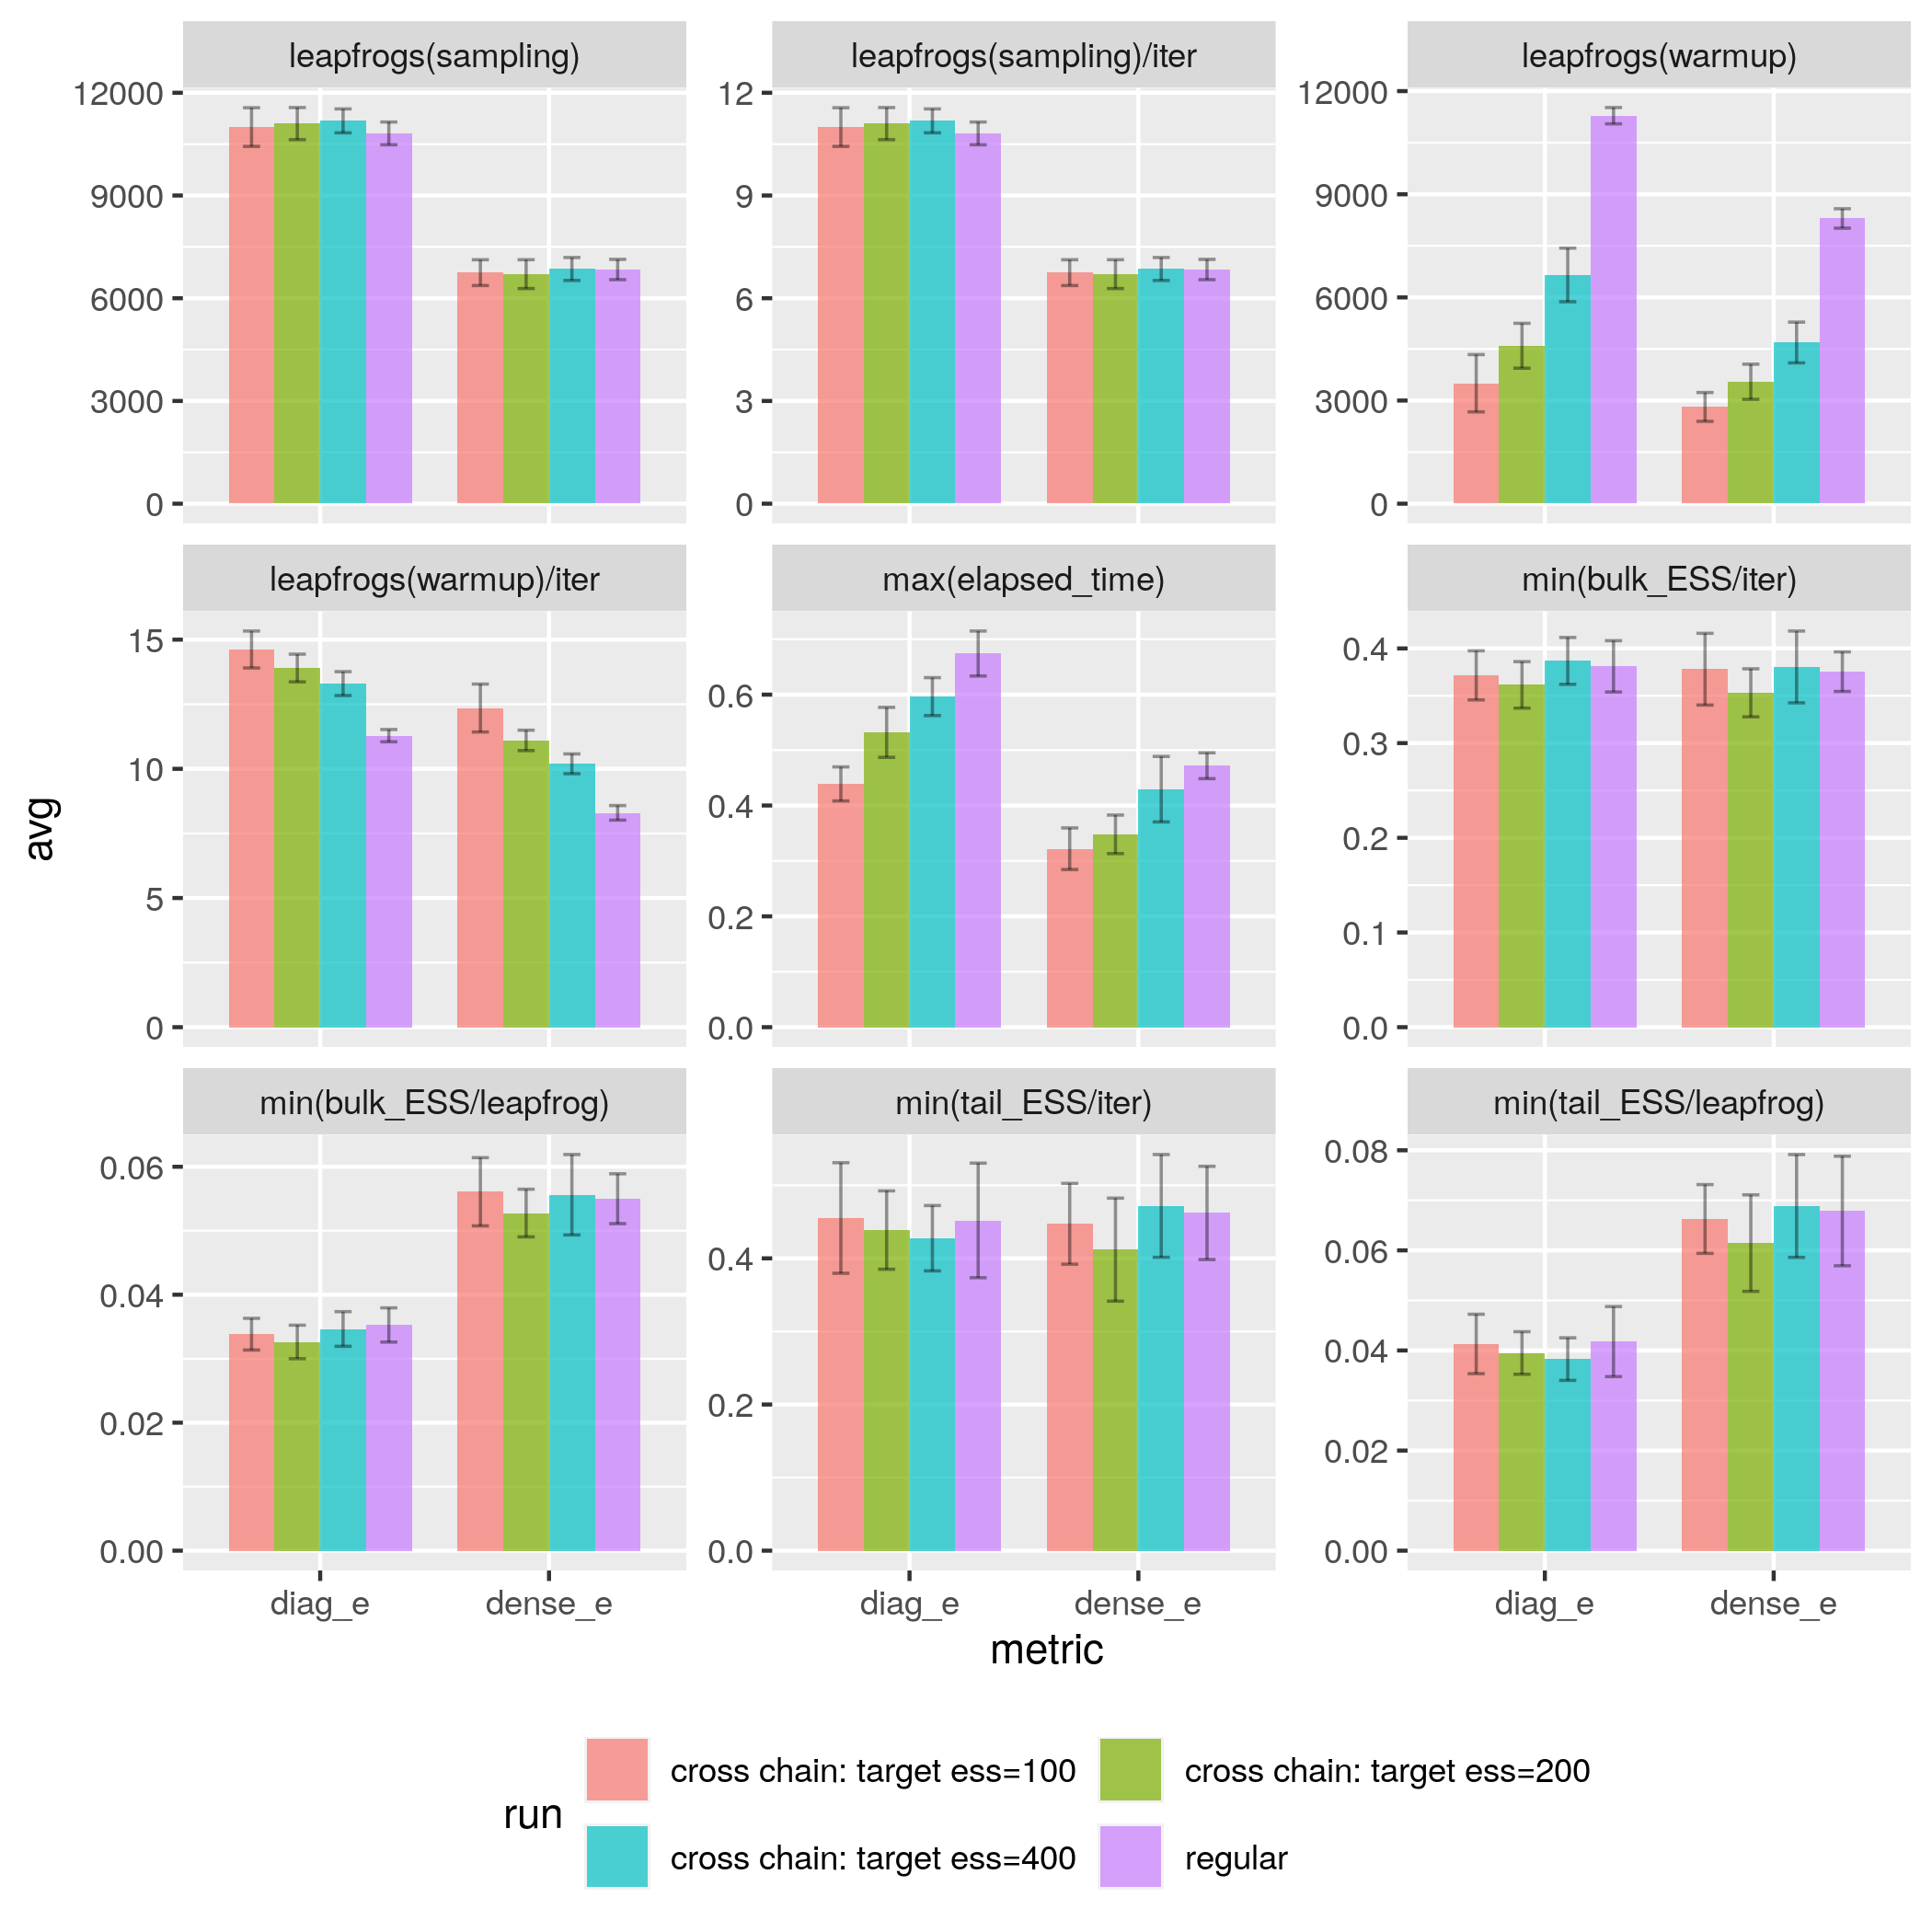
\includegraphics[width=\textwidth]{./figure/cross_chain_ess_effect_garch-garch11.png}
\caption{Cross-chain warmup performance comparison: garch-garch11 model}
\end{figure}

\begin{figure}[htbp]
\centering
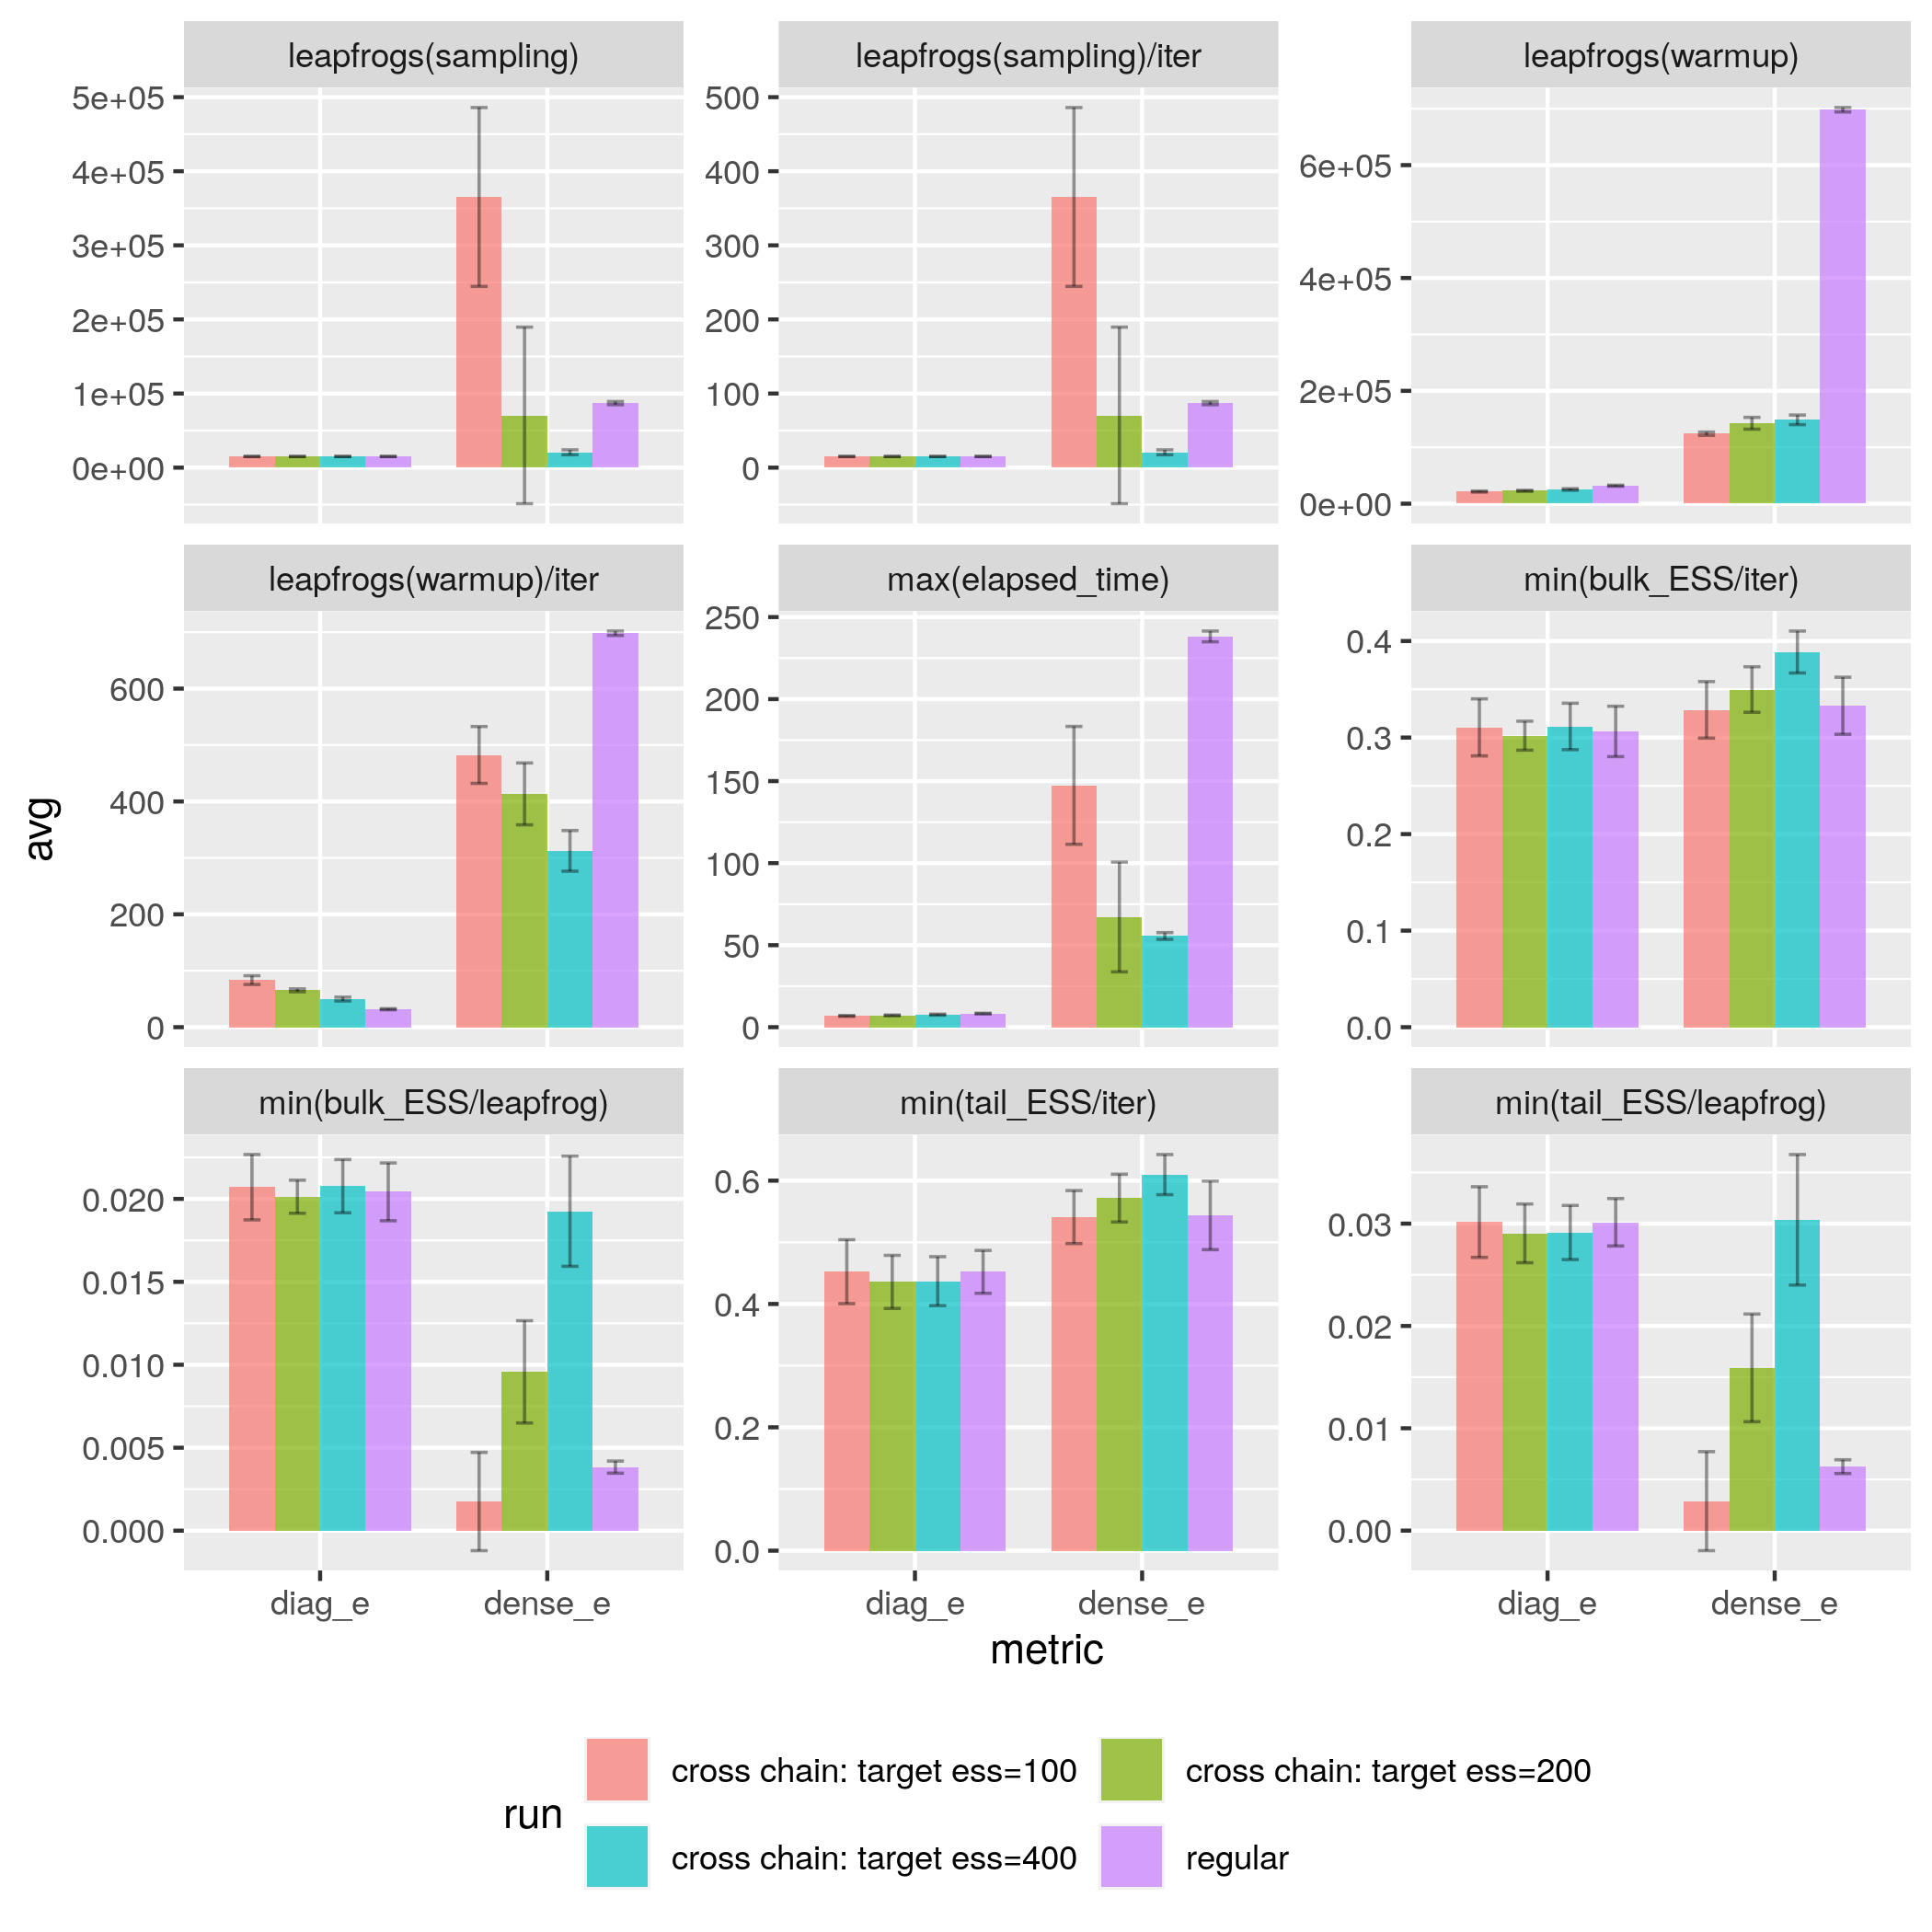
\includegraphics[width=\textwidth]{./figure/cross_chain_ess_effect_radon.png}
\caption{Cross-chain warmup performance comparison: radon model}
\end{figure}

\begin{figure}[htbp]
\centering
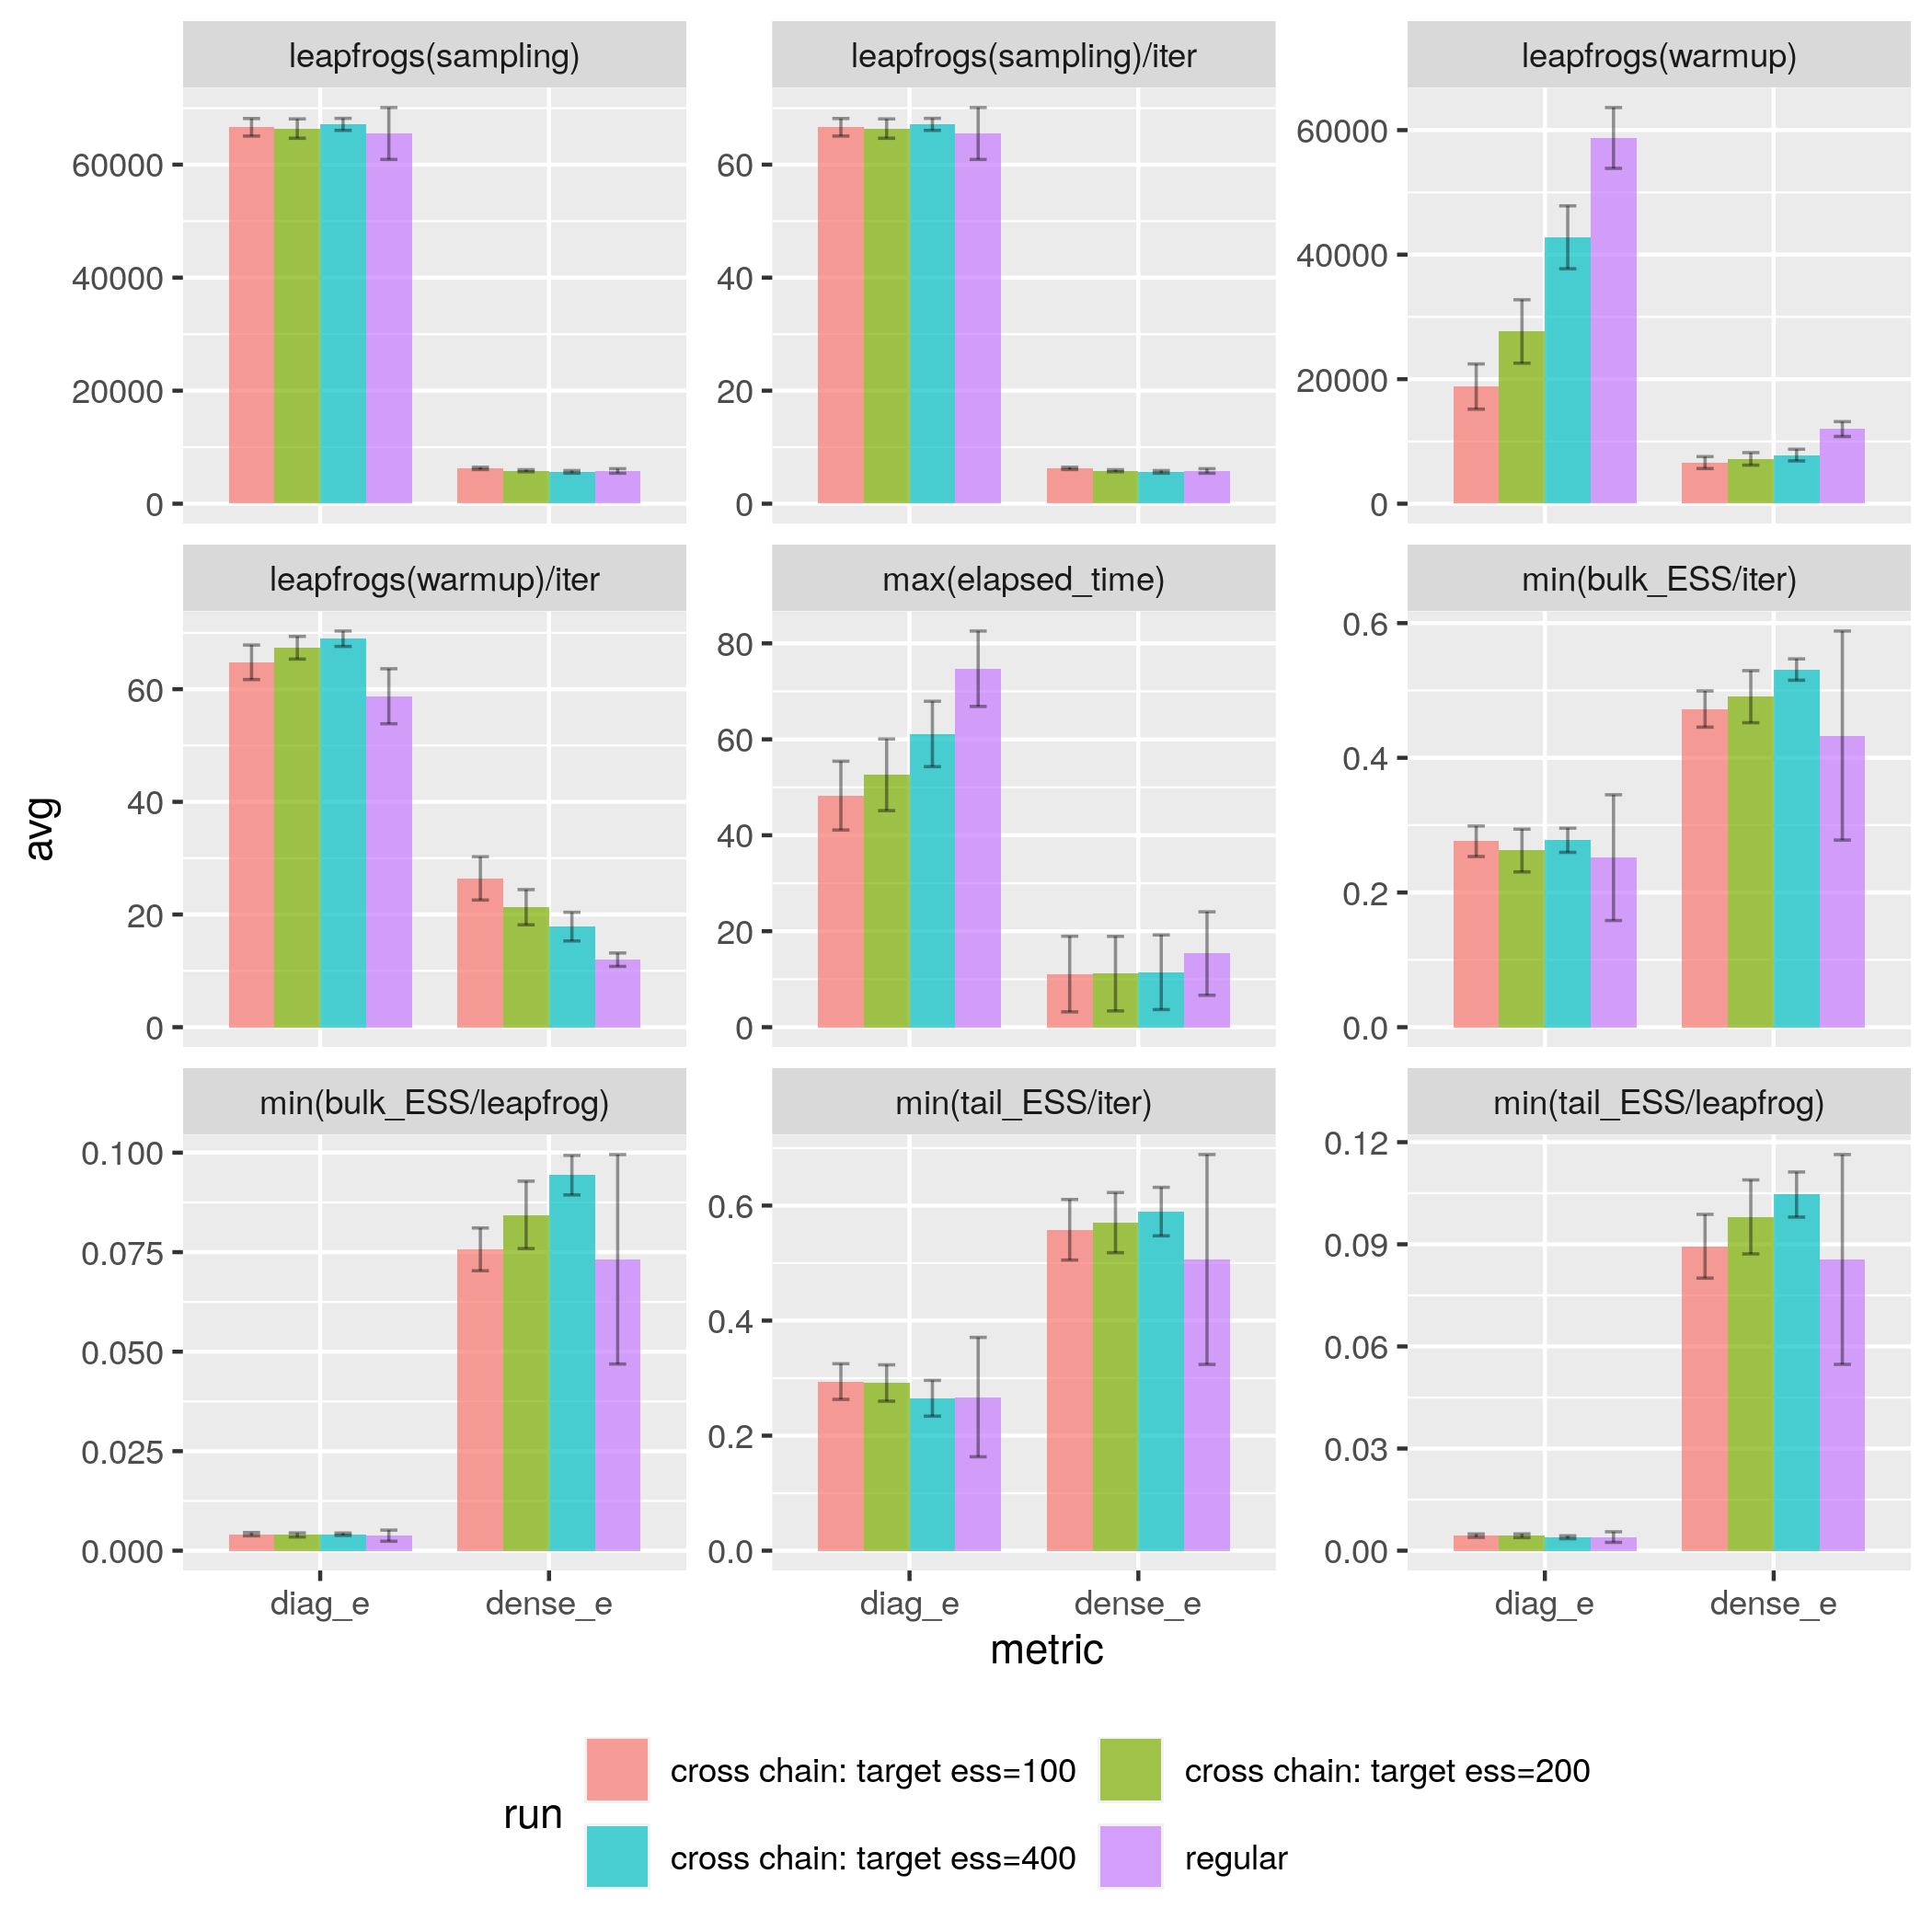
\includegraphics[width=\textwidth]{./figure/cross_chain_ess_effect_sir.png}
\caption{Cross-chain warmup performance comparison: SIR model}
\end{figure}

\begin{figure}[htbp]
\centering
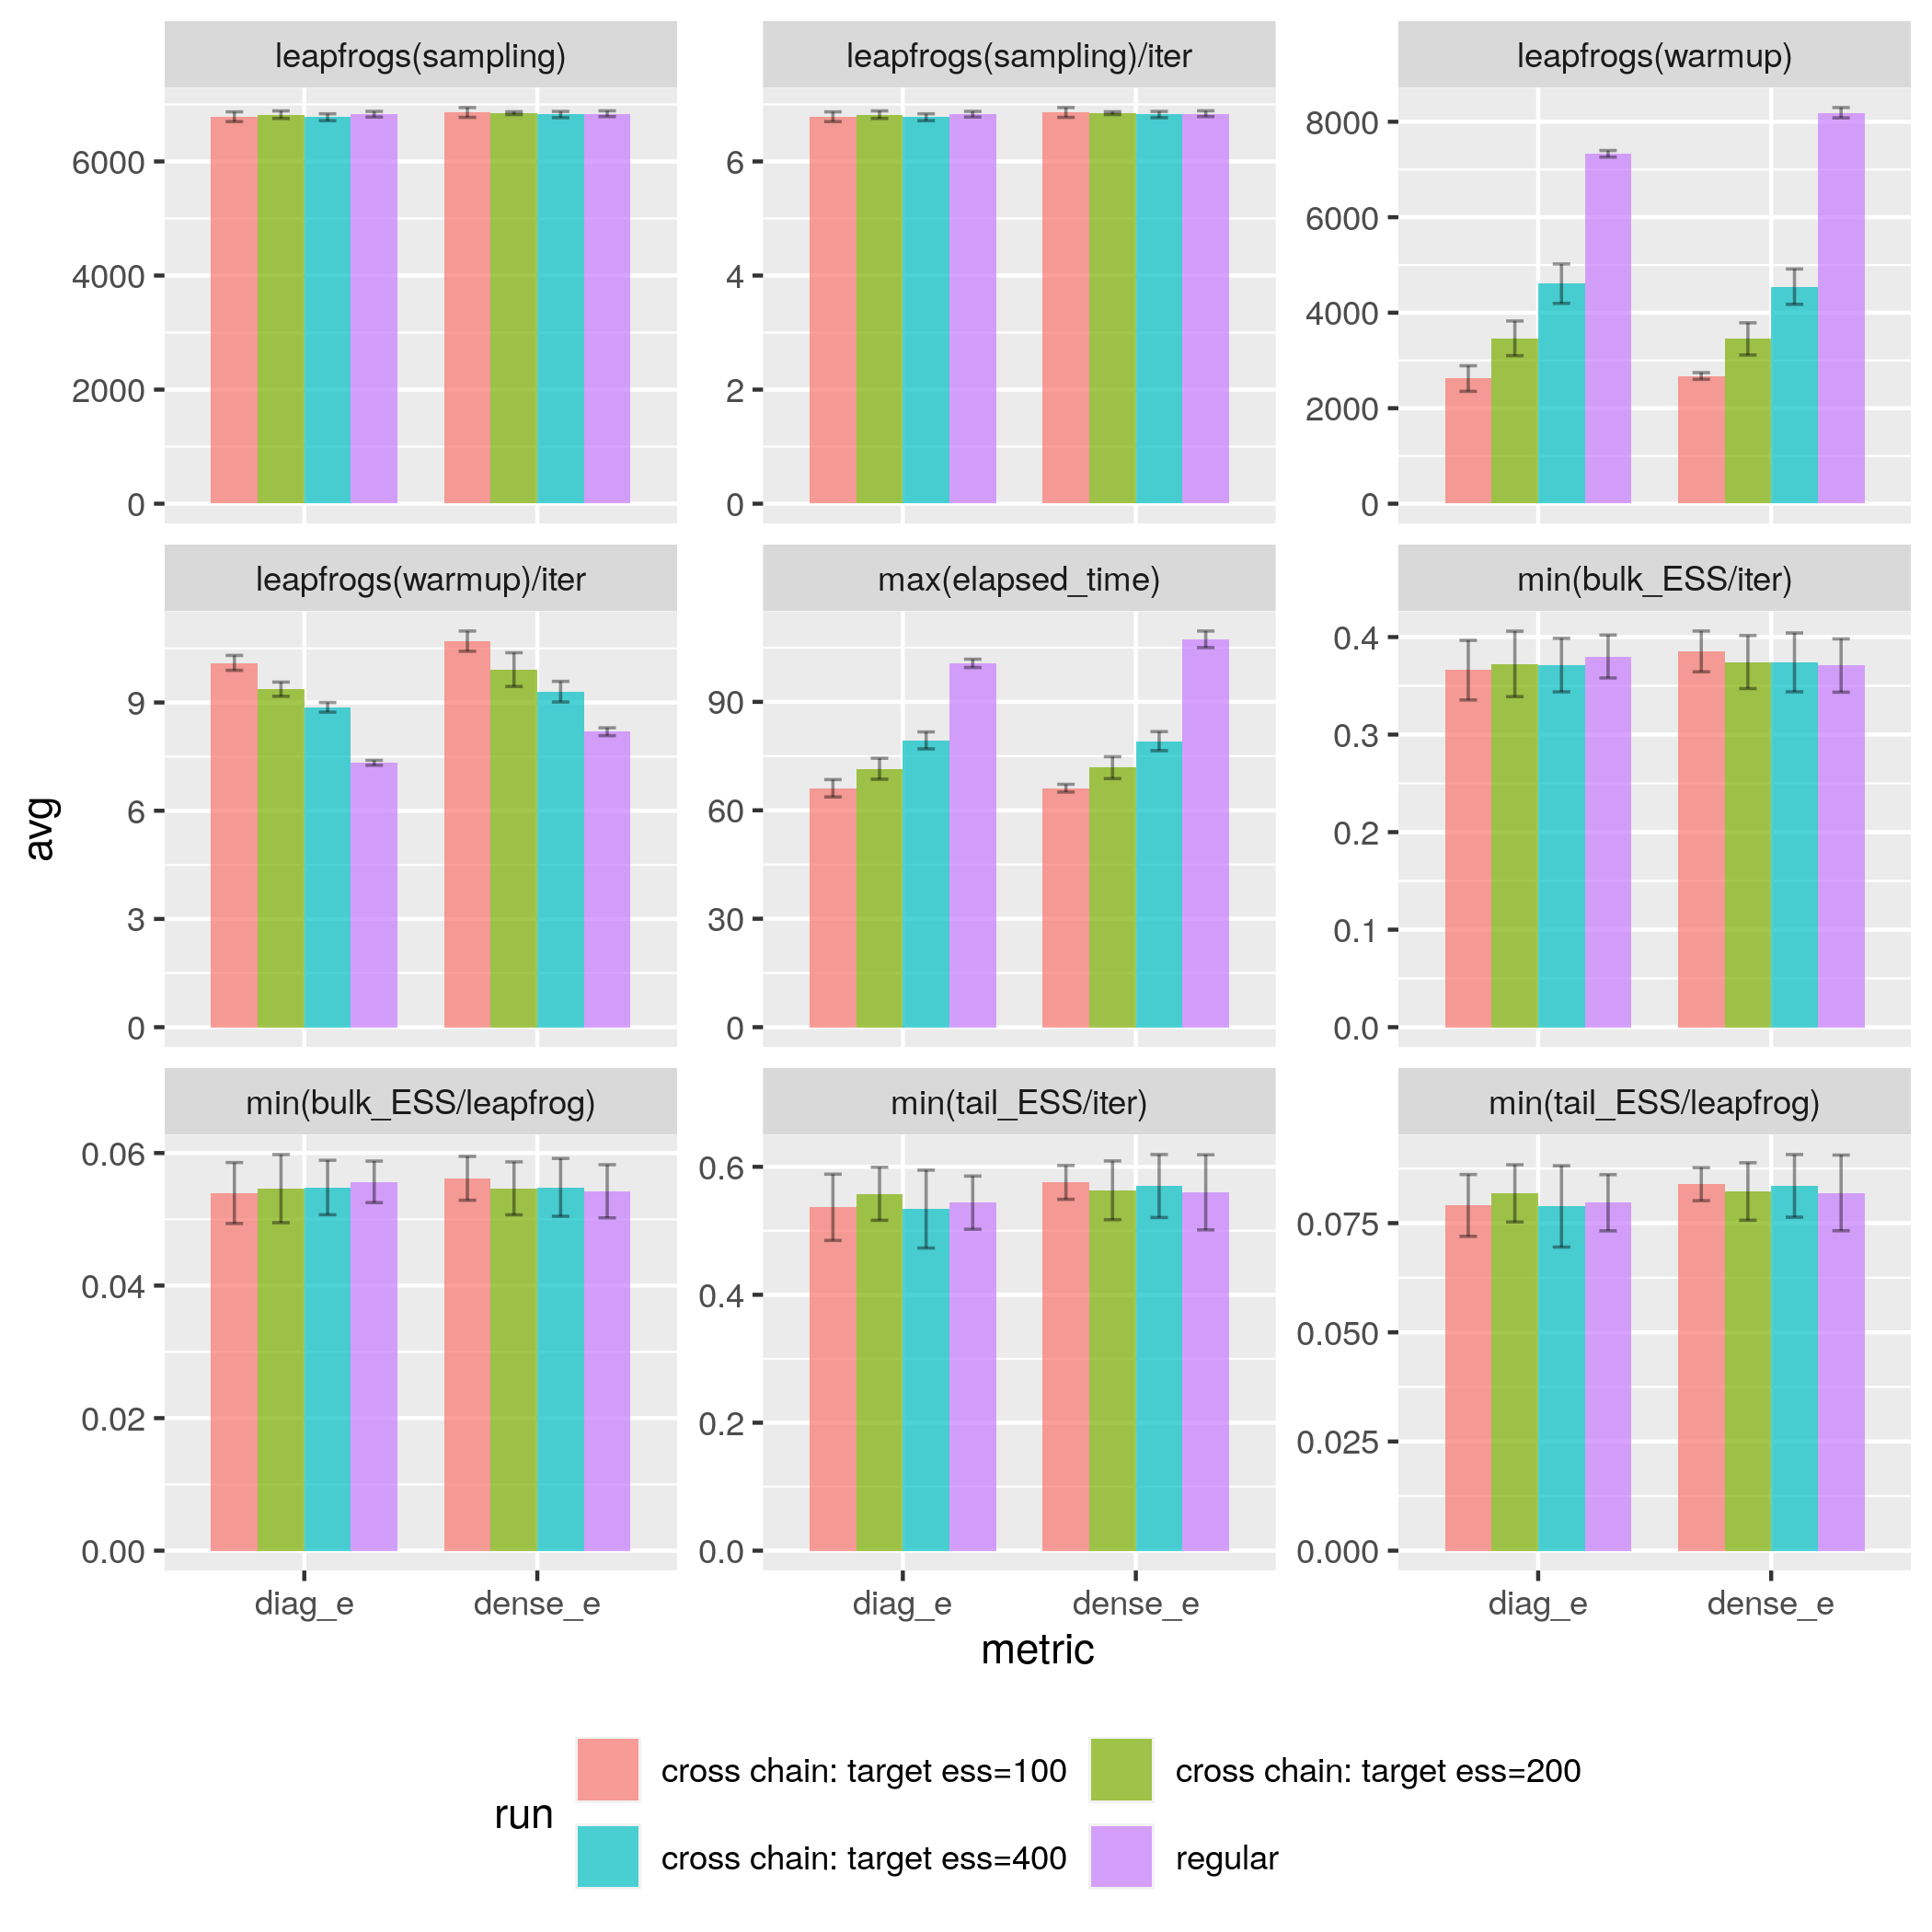
\includegraphics[width=\textwidth]{./figure/cross_chain_ess_effect_chem.png}
\caption{Cross-chain warmup performance comparison: chemical reaction model}
\end{figure}


\section{Multilevel parallelism: combining cross-chain warmup and within-chain parallelization}
\label{sec:orgf72ae3d}
Combining cross-chain warmup and
within-chain parallelization, we are able to design a framework of
\emph{multilevel parallelism} for Bayesian inference of population
models. Orthogonal to the above warmup algorithm, \emph{within-chain}
parallelization implemented in Stan
and Torsten does not induce communication across chains but distributes a
heavy-lifting modeling task to mutiple processes in a single
chain. In Torsten this within-chain strategy focuses on solving ODEs
in population model. The corresponding functions are \cite{torsten_pmx_group}
\begin{minted}[breaklines=true,fontsize=\footnotesize,breakanywhere=true]{stan}
pmx_solve_group_rk45
pmx_solve_group_adams
pmx_solve_group_bdf
\end{minted}

\subsection{Algorithm \& implementation}
\label{sec:org7d1fe53}
Our multilevel framework has an upper and lower level of parallelization(Figure \ref{multilevel-diagram}). The upper
level handles the cross-chain warmup by running parallel chains and
updating metric and stepsize. Chains exchange
information only at the end of each window at this level. 

The lower level of within-chain parallelization occurs more
frequently: with every new set of parameter samples, NUTS updates the likelihhod
by solving the ODEs in the population model, and Torsten's group
solvers distribute the population to multiple processes, with each
processe handling one or several subjects' ODE systems.

\begin{figure}[htbp]
\centering
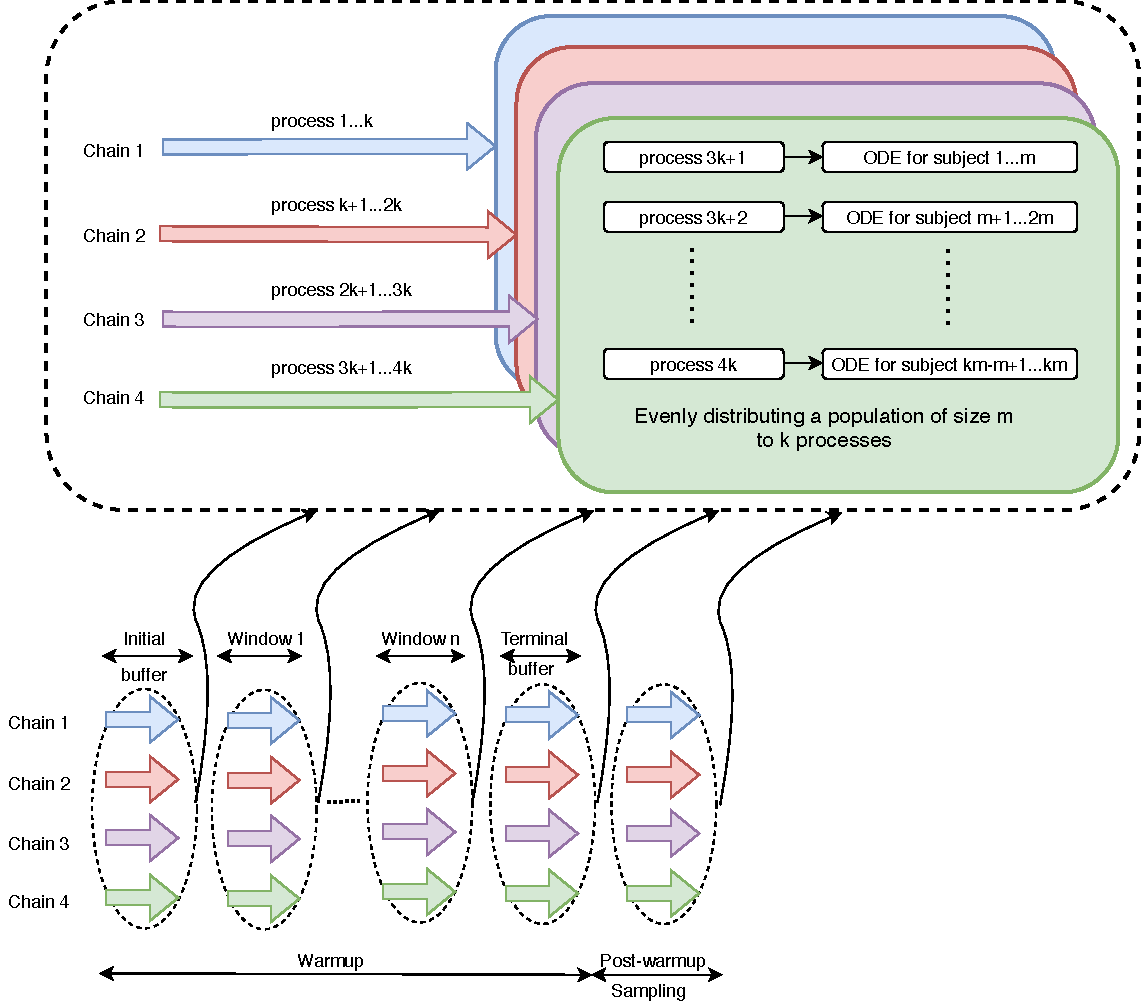
\includegraphics[width=\textwidth]{./figure/within_chain_parallel_diagram.pdf}
\caption{Multilevel parallelism for ODE-based population models. A simplified version of Figure 1, the lower diagram shows the cross-chain warmup through multiple windows. In within-chain parallelization, as shown in the upper diagram, each chain has its own parameter samples(indicated by different colors), and dedicated processes for solving the population model. \label{multilevel-diagram}}
\end{figure}

\subsection{Example}
\label{sec:orgadc9a94}
To demonstrate the above multilevel method, we apply it to a
time-to-event model for the time to the first grade 2+ peripheral neuropathy (PN)
event in patients treated with an antibody-drug conjugate (ADC)
delivering monomethyl auristatin E (MMAE). We call it
Time-To-PN(TTPN) model, and analyze data using a
simplified version of the model reported in
\cite{lu_time--event_2017}. We consider three treatment arms:
fauxlatuzumab vedotin 1.2, 1.8 and 2.4 mg/kg IV boluses q3w x 6 doses,
with 20 patients per treatment arm. In this model,
each patient's PK is described by an effective compartment model(one-compartment),
and PD by a linear model. The likelihood for time to first 2+ PN event
is described by a hazard function that depends on the concentration
effect through Weibull distribution. Two unknowns from
PK model and the cumulative hazard form a three-component
ODE system. Each evaluation of likelihood requires solving this
3-system for every patient. 

In Torsten's model, ODEs corresponding to the entire
population can be solved by a single call of \mintinline[breaklines=true,fontsize=\footnotesize,breakanywhere=true]{stan}{pmx_solve_group_rk45} function. The three parameters of the
model are:
\begin{itemize}
\item \(k_{e0}\) in effective compartment model.
\item \(\alpha\) the coefficient of linear PD model.
\item \(\beta\) Weibull distribution scale parameter.
\end{itemize}

To activate multilevel feature, compile model with \mintinline[breaklines=true,fontsize=\footnotesize,breakanywhere=true]{bash}{cmdstan/make/local} set as
\begin{minted}[breaklines=true,fontsize=\footnotesize,breakanywhere=true]{bash}
STANC2=true
TORSTEN_MPI=1
MPI_ADAPTED_WARMUP=1
TBB_CXX_TYPE=clang
\end{minted}
and run it with
\begin{minted}[breaklines=true,fontsize=\footnotesize,breakanywhere=true]{bash}
# we use MPICH options in this report.
mpiexec -n nproc -l -f hostfile ./model-name sample save_warmup=1 adapt cross_chain_ess=target_ess data file=model-name.data.R init=init.R random seed=seed id=i
\end{minted}

Similar to previous section, Figure shows performance of cross-chain and
regular runs based on target ESS = 400. Unlike in previous models, we
did not performe runs with multiple seed or target ESS to avoid long
computing time. One can make conclusion consistent with the other
models, that the cross-chain warmup reduce total run time without
compromising ESS.

\begin{figure}[htbp]
\centering
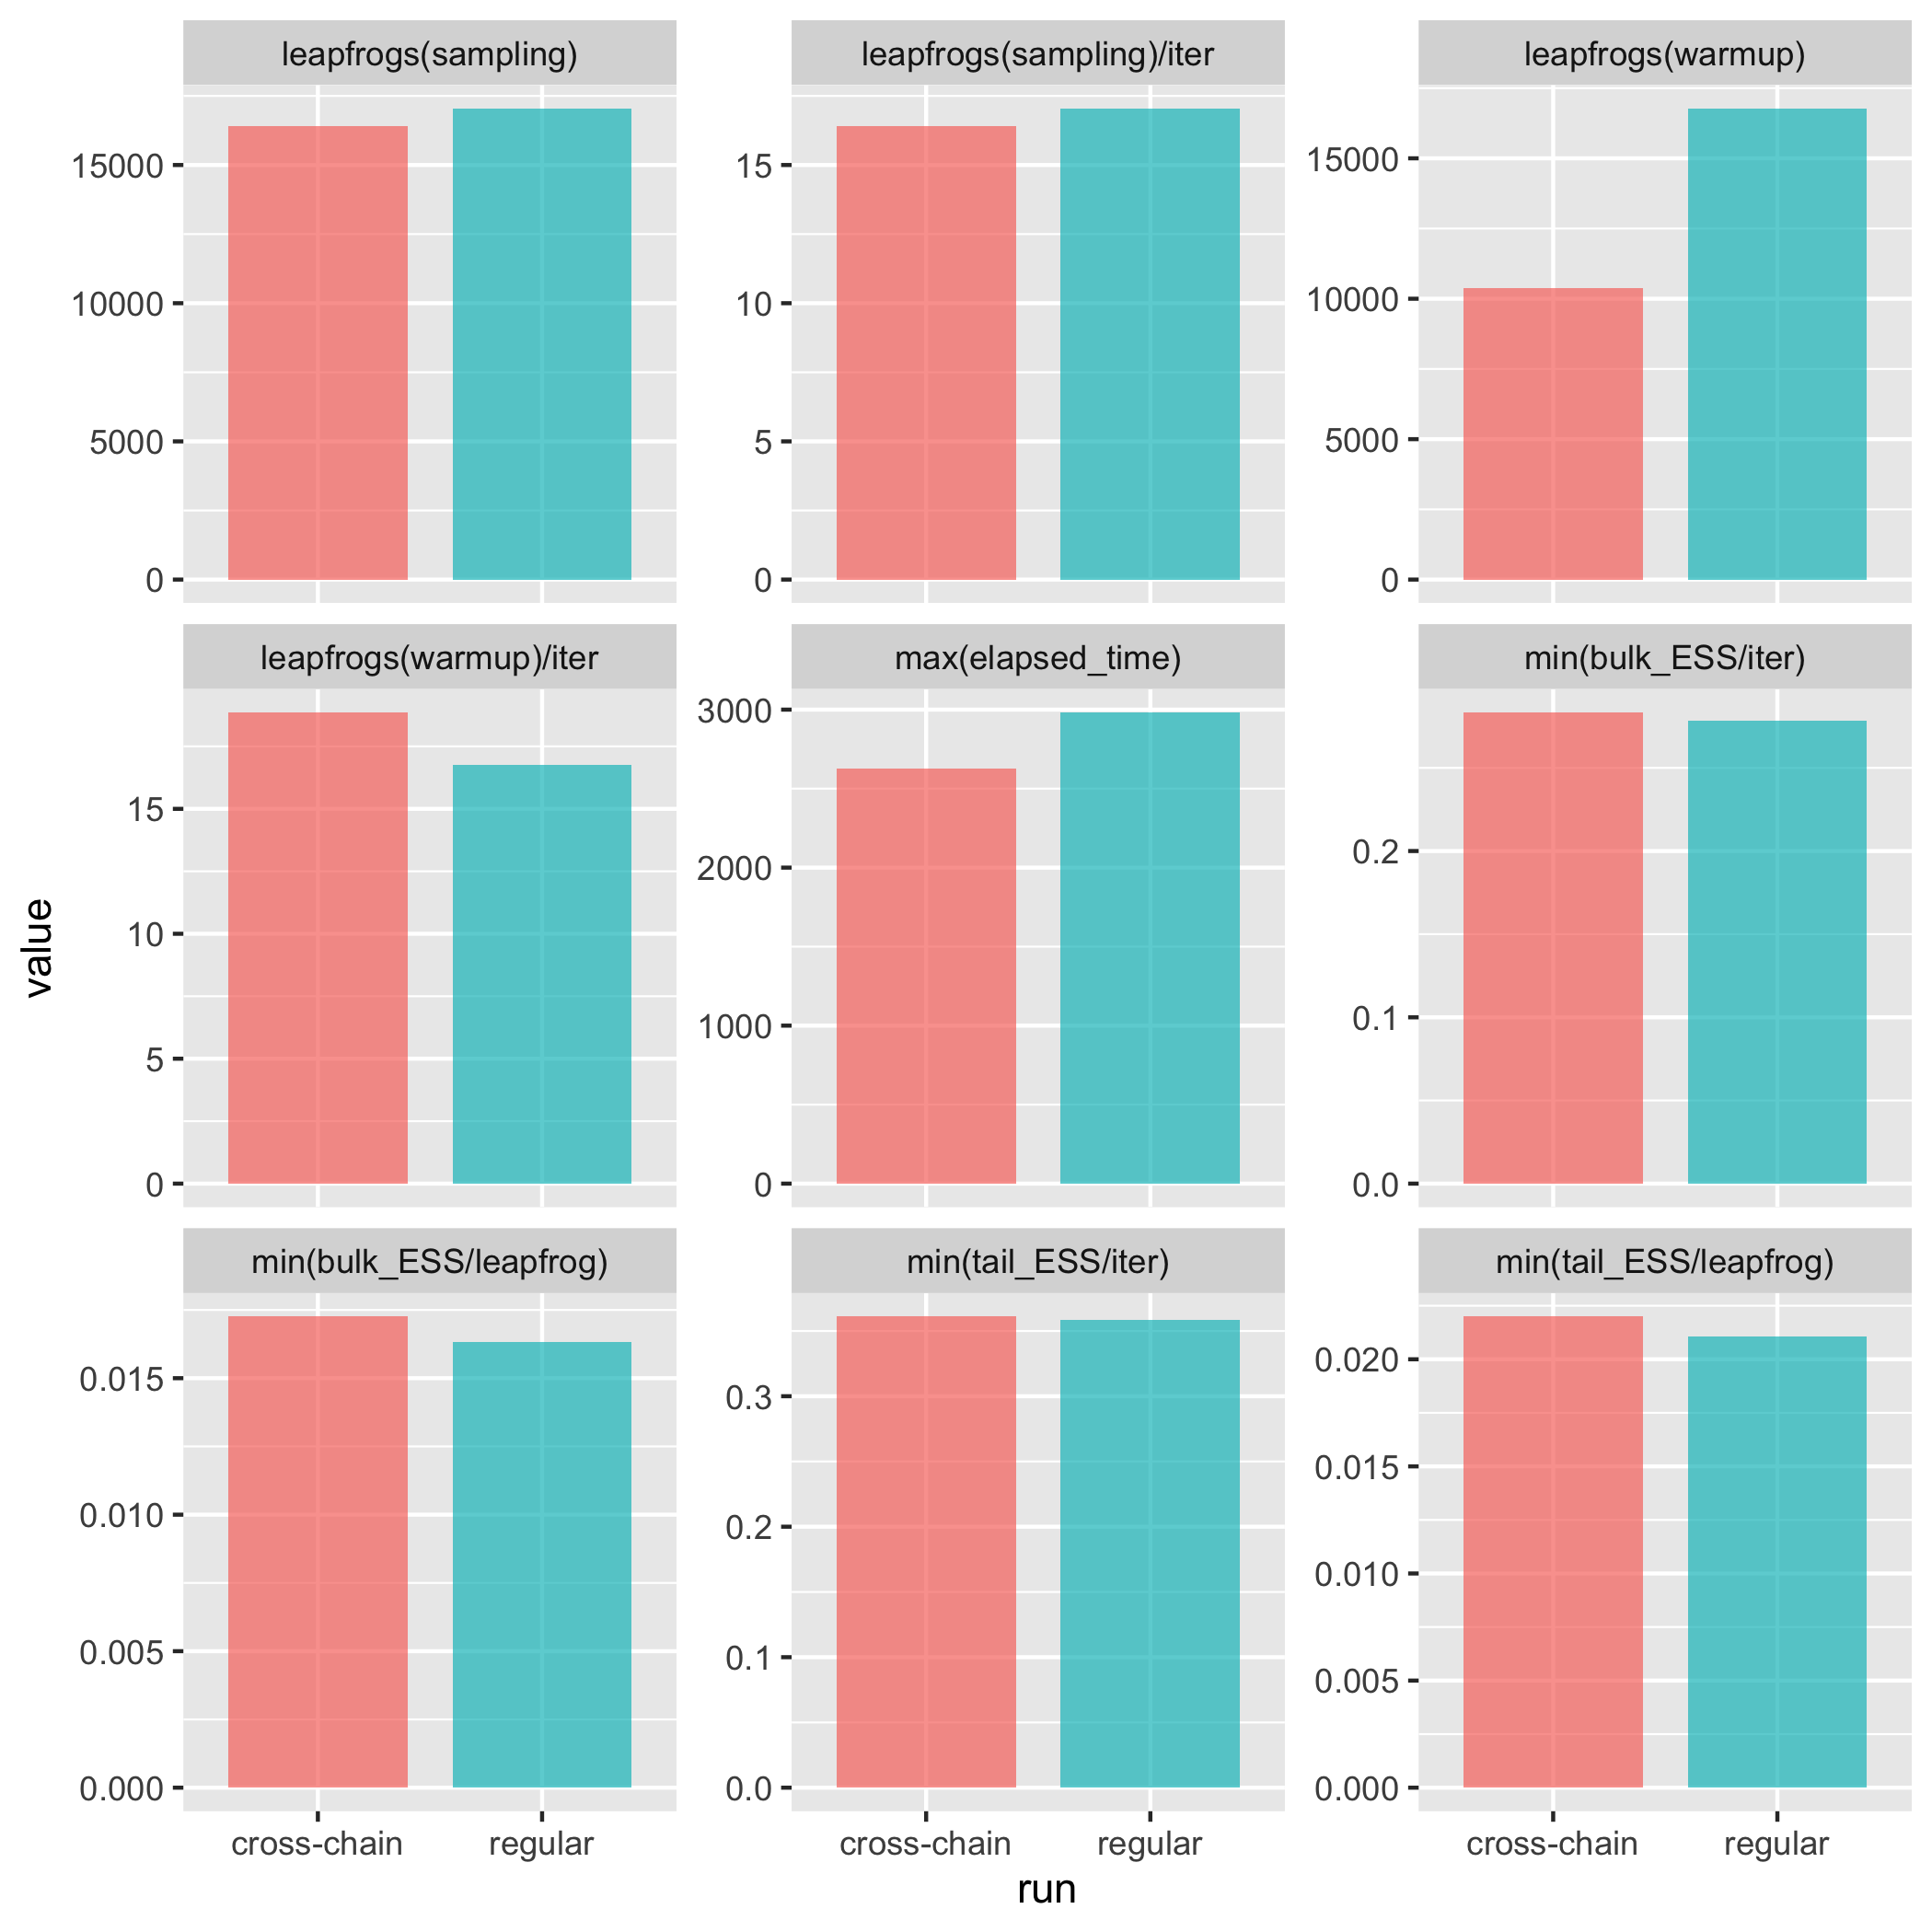
\includegraphics[width=\textwidth]{./figure/ttpn2_ess_400_cross_chain_vs_seq.png}
\caption{Cross-chain warmup performance comparison(Target ESS 400): TTPN model.}
\end{figure}

Next, we apply multilevel method to TTPN model with a fixed target ESS
= 400, by running the model
with 4 chains using \(n_{\text{proc}} = 8, 16, 32, 60, 80\)
processes. Equivalently, there are
\(n_{\text{proc\_per\_chain}} = 2, 4, 8, 15, 20\)
processes per chain so that within-chain parallelization can be utilized.
With population size 60, each process handles solution of
\(n_{\text{id}} = 30, 15, 7, 4, 3\)
subjects' ODE system, respectively.

To show parallel scaling performance, we collect \mintinline[breaklines=true,fontsize=\footnotesize,breakanywhere=true]{c}{stanfit} objects of the benchmark runs
and plot their wall time speedup against regular Stan runs. With all
runs having 1000 post-warmup sampling iterations, in
multilevel runs the number of warmup iterations is determinted at
runtime, while both within-chain parallel runs and regular Stan runs
have 1000 warmup iterations. Among 4 chains in a run, we use the
one with maximum total walltime(in seconds) as performance measure, as
in practice usually further model evaluation becomes accessible only
after all chains finish.

As shown in Figure \ref{cc-diagram}, both muiltilevel and
within-chai-only parallel runs exhibit good scaling up to 60
processes(15 processes per chain \(\times\) 4 chains)\footnote{We did not apply more than 60 processes in benchmark in order
to reduce cluster computing cost in this study. Previous study on within-chain parallelization
\cite{torsten_pmx_group} shows that reward of using more cores
diminishes.}. In
addition, cross-chain warmup enables multilevel runs to be more
efficient, with a steady \textasciitilde{}20\% performance gain when 4+ processes per
chain are applied. Since two parallel setup produce similar
post-warmup sampling efficiency, this gain is entirely contributed by
our new warmup algorithm.

\begin{figure}[htbp]
\centering
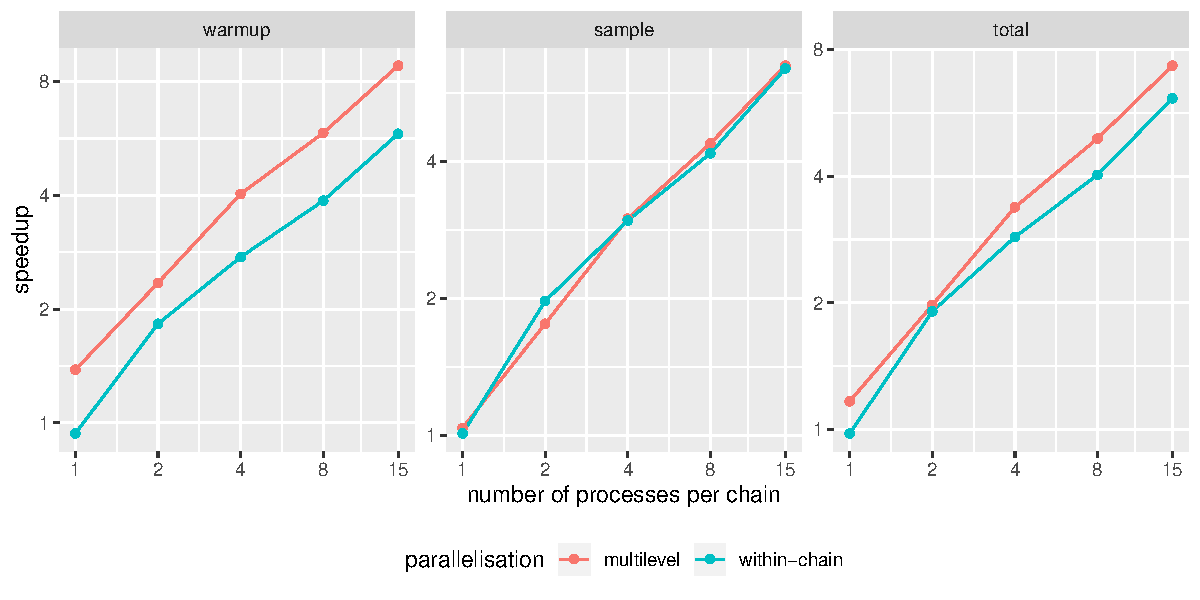
\includegraphics[width=\textwidth]{./figure/ttpn2_perf_benchmark.pdf}
\caption{multilevel parallelisation performance of TTPN model(target ESS=400). Speedup for warmup, sampling, and total(warmup + sampling) are based on corresponding regular run wall time. \label{ttpn_perf}}
\end{figure}

\section{Conclusion}
\label{sec:org25e5b88}
Multilevel parallelism using in Stan and Torsten
significantly improves computational efficiency and extends
the range of models that may be practically implemented.

\bibliography{torsten}
\bibliographystyle{siam}
\end{document}
